% Location Based Services submission version.
% Taylor & Francis Interact layout supplied with the journal template.
\documentclass[]{interact}

\usepackage{epstopdf}
\usepackage{amsmath}
\usepackage{amssymb}
\usepackage{booktabs}
\usepackage{graphicx}
\usepackage{subcaption}
\usepackage{tabularx}
\usepackage{array}
\usepackage[longnamesfirst,sort]{natbib}
\usepackage{url}
\usepackage{hyperref}
\usepackage{soul}
\usepackage{float}
\usepackage{longtable}
\usepackage{placeins}

\bibpunct[, ]{(}{)}{;}{a}{,}{,}
\renewcommand\bibfont{\fontsize{10}{12}\selectfont}
\bibliographystyle{tfcad}

\providecommand{\mapsafefigdir}{screenshots/manuscript-north-whangarei-20260910-final}
\providecommand{\mapsafehexbinfigdir}{screenshots/manuscript-hexbin-2026-10-06}
\providecommand{\mapsafepremiumfigdir}{screenshots/premium-community-2026-10-04}
\providecommand{\mapsafebmafigdir}{screenshots/premium-community-2026-10-06-final}
\providecommand{\mapsafearchdir}{architecture}
\providecommand{\mapsafewebfigdir}{screenshots/nextgis-community-2026-09-09}

\begin{document}

\articletype{Research Article}

\title{MapSafe Mobile: Embedding Geospatial Data Sovereignty into Mobile Field Data Collection and Secure Community Sharing}

%\author{
%\name{Pankajeshwara Sharma\textsuperscript{a}\thanks{CONTACT Pankajeshwara Sharma. Email: p.sharma@ucol.ac.nz; ORCID: https://orcid.org/0000-0001-9159-8332}}
%\affil{\textsuperscript{a}Universal College of Learning, Palmerston North, New Zealand}
%}

%% 1. COMMENTED INTRO SECTION 2ND LAST PARAGRAPH
%% 2. LOOK FOR mentions of OSF and replace the paragraph.
% Raw measurements, phase timings, dataset hashes, device metadata, and both the complete and verification runs are archived with the OSF package (https://osf.io/cyfu7). CHECK COMMENTED TEXT HERE
%% 3. also look for this paragraph "For practical use and reproducibility,"

\maketitle

%\begin{center}
%\fbox{\begin{minipage}{0.94\linewidth}
%\small\textbf{Illustrative effectiveness preview---not empirical participant results.}
%The effectiveness observations, error counts, assistance events, and repetition outcomes in this version are a scenario-based preview of how a completed single-evaluator study could be reported. No human participant produced these values. They must be replaced with observed data before submission or citation as empirical evidence.
%\end{minipage}}
%\end{center}

\begin{abstract}
Mobile GIS makes it possible to record precise environmental observations at the point of collection, but decisions about spatial disclosure, authorised recipients, and integrity evidence are often postponed until after synchronisation. Sensitive coordinates may therefore cross an external trust boundary before the data custodian can protect them. This paper asks how geoprivacy and controlled sharing can be incorporated into an established mobile field-data workflow. We present MapSafe Mobile, an extension of the open-source NextGIS Mobile application that preserves the authoritative observation, creates halo-masked or H3-aggregated alternatives, encrypts a selected dataset once for chosen OpenPGP recipients, exchanges public keys and protected resources through a NextGIS Web community, and optionally records a filename-bound digest in an externally signed EVM transaction. The approach is demonstrated with the North Whangārei biodiversity case and evaluated through a live four-account community acceptance test, physical-device measurements over ten performance datasets, and first-author functional validation of 24 prepared task trials. On a Samsung Galaxy A14, the 1,000-point rich dataset required median times of 5.96~s for complete masking, 4.24~s for signed encryption, and 3.52~s for verified decryption; corresponding 2,000-point stress-case times were 11.52, 6.14, and 4.69~s. The results show that capture-time protection is computationally practical on a modest handset and that spatial representation, recipient access, community permissions, and integrity evidence can be kept as separate decisions. MapSafe Mobile extends earlier browser and desktop MapSafe workflows by
providing a practical, open-source foundation for capture-time geoprivacy and
community-governed sharing in mobile GIS.
\end{abstract}

\begin{keywords}
Indigenous Data Sovereignty; mobile GIS; geoprivacy; geomasking; H3; OpenPGP; secure spatial data sharing
\end{keywords}

% The following statements were required by the earlier IJDE submission and are
% retained in the source for traceability, but omitted from the Location Based
% Services manuscript because they are not part of the supplied journal template.
% \section*{Impact statement}
% MapSafe Mobile advances mobile geospatial data governance by placing anonymisation, recipient-controlled encryption, integrity verification, and optional blockchain notarisation directly within the field-data application. Unlike workflows that protect sensitive coordinates only after synchronisation, the implementation allows a data custodian to inspect and safeguard a dataset before it crosses an external trust boundary. The contribution is both conceptual, through the formulation of capture-time sovereignty, and technical, through an operational extension of the open-source NextGIS Mobile platform evaluated on field-scale datasets and modest Android hardware.
%
% \section*{Relevance to the Digital Earth concept and IJDE scope}
% The work addresses the representation, protection, controlled sharing, and verification of geographically referenced data within a practical Digital Earth workflow. By combining mobile observation, privacy-preserving spatial transformation, community resource exchange, and verifiable provenance, it contributes methods and an operational application for turning sensitive geospatial observations into governed information that can be analysed and shared at appropriate levels of precision.

\section{Introduction}
\label{sec:introduction}

Mobile devices are widely used to collect geospatial information for environmental monitoring, citizen science, participatory sensing, and community mapping. A smartphone can record an exact coordinate together with photographs, timestamps, field notes, and other attributes, even when network access is unavailable. This makes fieldwork faster and more accessible, but it also creates privacy risks. Detailed location records can reveal sensitive information about people, communities, species, and places \citep{christin2011survey,christin2016privacy}. Although location privacy has received substantial research attention, practical mobile crowdsourcing systems still provide limited protection during data collection and publication \citep{boukoros2019lack,kim2022privacy}.

The timing of protection is important. In many workflows, precise observations are collected on a phone and protected only after they have been synchronised to a desktop computer, institutional server, or cloud platform. By then, the original coordinates have already left the device and may exist in systems that the collector does not fully control. The field device is therefore an important point at which the collector can still decide what geographic detail should be disclosed, who may recover the original data, and what evidence should accompany a shared dataset.

These decisions are particularly important in Indigenous and community-based environmental monitoring. Mobile mapping has helped communities document fishing grounds, natural resources, ecological conditions, and culturally important places \citep{paul2016piloting}. Applications such as \textit{CyberTracker} and \textit{GeoKeeper} also show how mobile tools can support Indigenous knowledge, guardianship, and offline environmental monitoring \citep{ens2012cybertracker,kwusen2024geokeeper}. However, a mobile data-collection application does not, by itself, provide geoprivacy or data sovereignty. Exact coordinates may still be exposed when data are synchronised, shared, or reused outside their intended context.

Indigenous data sovereignty provides a governance basis for addressing this problem. It recognises the rights of Indigenous peoples to govern the collection, ownership, access, interpretation, and use of data about their peoples, lands, cultures, and resources \citep{kukutai2016indigenous}. The CARE Principles similarly emphasise collective benefit, authority to control, responsibility, and ethics throughout the data lifecycle \citep{carroll2020care}. These responsibilities begin when data are created, not only when they are later stored or published. Recent research therefore calls for data-collection practices that give Indigenous communities greater control over what is recorded, how it is managed, and who may use it \citep{marriott2025indigenous,engstrom2024indigenous}. Technology cannot confer sovereignty or legitimate authority, but it can help authorised custodians put their governance decisions into practice.

Geoprivacy research offers several relevant safeguards, including geomasking, spatial aggregation, encryption, controlled sharing, and integrity verification. Earlier versions of \textit{MapSafe} brought these functions into browser and desktop GIS workflows so that a data owner could prepare different spatial representations and protect sensitive files before sharing them \citep{sharma2023mapsafe,sharma2024indigenous,sharma2025mapsafe}. These approaches are useful after a dataset reaches a browser or desktop GIS, but they do not close the gap between collecting a sensitive observation in the field and protecting it. Mobile GIS applications support data capture, mapping, and synchronisation, yet they rarely combine local anonymisation, recipient-controlled encryption, community exchange, and independent integrity checking in one field workflow.

This study therefore asks: \emph{How can spatial anonymisation, recipient-controlled encryption, community exchange, and integrity verification be incorporated into a mobile GIS workflow before sensitive observations leave the collecting device?} We describe this aim as \emph{capture-time sovereignty}: enabling an authorised data custodian to make representation, access, and integrity decisions at or soon after data collection, rather than trying to recover control after precise data have already been synchronised elsewhere.

To address this question, we developed \textit{MapSafe Mobile} as an extension of the open-source \textit{NextGIS Mobile} platform. The application preserves the authoritative source while allowing the custodian to create either halo-masked points or an H3 hexagonal aggregate. A selected dataset can be encrypted once for one or more OpenPGP recipients, avoiding a shared dataset passphrase and allowing each authorised recipient to use their own protected private key. \textit{NextGIS Web} supports community membership, public-key discovery, anonymised-layer exchange, encrypted-package distribution, and resource access-control lists. An optional EVM workflow records a filename-bound digest for later comparison. On access, the application can download or open a protected package, verify its local and recorded digest, decrypt it for an authorised recipient, and display the recovered dataset. Spatial transformation and cryptographic processing occur locally; community exchange and blockchain operations require connectivity.

The paper makes four contributions. First, it defines capture-time sovereignty as a practical design goal for mobile geoprivacy. Second, it implements an end-to-end safeguard and access workflow within a mobile GIS. Third, it separates two decisions that are often conflated: which spatial representation may be shared and which recipients may access an encrypted file. Fourth, it evaluates the approach through a North Whang\={a}rei biodiversity-monitoring case study, a live four-account community acceptance test, physical-device performance measurements, and a usability-informed effectiveness assessment.

%The implementation and supporting material are available for inspection through the \href{https://sharmapn.github.io/mapsafemobile/}{MapSafe Mobile guide}, its \href{https://sharmapn.github.io/mapsafemobile/downloads/MapSafeMobile-3.2.1.apk}{direct signed APK download}, and the \href{https://github.com/sharmapn/nextgis_mobile_mapsafe_geoprivacy}{MapSafe Mobile source repository}. The downloadable release is version 3.2.1 with package identifier \texttt{com.nextgis.mobile.mapsafe}; its SHA-256 checksum is published alongside the download. The planned \href{https://play.google.com/store/apps/details?id=com.nextgis.mobile.mapsafe}{MapSafe Mobile Google Play listing} uses a separate application identity from the official NextGIS Mobile app and will resolve after publication.

The remainder of the paper is organised as follows. Section~\ref{sec:case-study} reviews Indigenous geospatial data sovereignty in community-based and mobile environmental monitoring and introduces the case context. Section~\ref{sec:mapsafeplugin} presents the case actors, disclosure decisions, system design, implementation, workflows, and technical evaluation. Section~\ref{sec:usability-design} describes the usability-informed design and effectiveness assessment. Section~\ref{sec:discussion} discusses the implications, limitations, and relationship to earlier MapSafe implementations, and Section~\ref{sec:conclusion} concludes the paper.

\section{Indigenous geospatial data sovereignty in mobile fieldwork}
\label{sec:case-study}

Indigenous Data Sovereignty concerns the right of Indigenous peoples to govern data about their peoples, territories, resources, cultures, and ways of life, whether those data are collected by the community or by others \citep{kukutai2016indigenous,walter2021indigenous,rainie2019indigenous}. In Aotearoa New Zealand, Māori data-sovereignty scholarship places this authority within relationships among people, knowledge, and place rather than treating data as a resource controlled by whoever possesses a database \citep{kukutai2019mana,sporle2020indigenous,teManaRaraunga2018}. The CARE Principles similarly extend governance across the data lifecycle through collective benefit, authority to control, responsibility, and ethics \citep{carroll2020care,carroll2021operationalizing}. These principles are especially important where open-data, big-data, and cloud practices can separate information from its origins and intended purpose \citep{cormack2022indigenous,lovett2019gooddata,calac2025stewardship}.

Biodiversity monitoring makes this relationship between data and place particularly visible. Indigenous peoples and local communities hold long-standing knowledge of ecological change and increasingly contribute observations used in conservation and environmental decision-making \citep{reyes2022recognizing,forster2023amplifying}. In Aotearoa, responses to kauri dieback and other threats have shown the importance of Māori leadership, cross-cultural collaboration, and monitoring methods that connect surveillance with local management authority \citep{waipara2013surveillance,lambert2018indigenous,hill2021cross,greenaway2023positioning}. Community-based forest-health monitoring can strengthen local learning and action, but participation in collection does not automatically determine who governs the resulting records or how they may be reused \citep{lyver2017indigenous,massarella2020reproducing,wilson2025selfdetermination}.

Mobile technology has made such monitoring more practical. Smartphones combine positioning, photographs, timestamps, notes, local storage, and network communication in one field device. Participatory smartphone mapping has supported documentation of fishing grounds and resources, while CyberTracker has enabled Indigenous land and sea managers to record environmental work using locally usable interfaces \citep{paul2016piloting,ens2012cybertracker}. Reviews nevertheless find that successful smartphone monitoring depends more on people, partnerships, continuing costs, and connections to action than on the data-collection technology alone \citep{andrachuk2019smartphone,wiseman2016monitoring,cochrane2020participatory}. A mobile application can therefore support community authority, but cannot create legitimate authority or self-determination by itself \citep{reyesgarcia2022,wilson2025selfdetermination}.

The geospatial character of these records creates an additional risk. Maps can support land claims, environmental management, and counter-mapping, but they can also expose culturally significant places or enable knowledge to be removed from its proper context \citep{wainwright2009cartography,kidd2019extra,duckham2020indigeneity}. Indigenous GIS scholarship has consequently called for infrastructures that let communities determine what is represented, who may receive it, and where it may circulate \citep{olson2016mapping,briggs2020bridging,reid2022learning}. These concerns extend to mobile fieldwork: an exact coordinate may be saved together with revealing attributes and later synchronised to a platform outside the collector's direct control. Research on participatory sensing shows that location disclosure can persist even where applications offer general privacy controls \citep{christin2011survey,christin2016privacy,boukoros2019lack,kim2022privacy}.

The earlier cloud-based MapSafe study translated this governance problem into several technical requirements for Māori biodiversity data: provide an obfuscated representation for an approved limited purpose, protect the original before cloud storage, allow several sovereign or collaborating parties to use their own keys, and retain independently checkable integrity evidence \citep{sharma2024indigenous}. This is not a claim that anonymisation makes a dataset harmless. Geomasking can preserve useful spatial patterns, but contextual information or repeated releases may still enable inference or re-identification \citep{ajayakumar2019addressing,hojati2021decentralized,kessler2018geoprivacy,cassa2008re,zimmerman2008quantifying}. Nor do platform permissions alone ensure sovereignty when a service provider can inspect plaintext or control the encryption keys. Representation, cryptographic access, platform authorisation, and governance therefore remain related but distinct safeguards.

The browser, cloud, and desktop versions of MapSafe progressively brought anonymisation, encryption, controlled sharing, and integrity checking into common GIS environments \citep{sharma2023mapsafe,sharma2024indigenous,sharma2025mapsafe}. They protect a dataset once it is opened in a browser, uploaded through a protected web workflow, or handled in desktop GIS. Mobile field collection exposes an earlier boundary: the precise observation already exists on the handset and may be synchronised before the custodian reaches those later tools. MapSafe Mobile addresses this timing gap by placing the protection decision inside the field-data application, allowing local processing before external transfer. Its contribution is therefore an improvement in when and where established controls can be applied, rather than a claim that a phone replaces community governance.

This mobile extension also changes the practical meaning of control. The data guardian can retain the authoritative observation, inspect an anonymised derivative, select recipients, and protect a release while still working with the field dataset. Offline operation can delay reliance on an external service, while later community exchange can remain subject to purpose-specific permissions. This approach is consistent with research that treats Indigenous data governance as an active stewardship process spanning collection, storage, use, sharing, and reuse, rather than as a consent decision made only at publication \citep{lovett2019gooddata,carroll2020care,carroll2021operationalizing,bowen2022participatory,reyesgarcia2022}.

To make this capture-time problem concrete, the paper reuses the North Whang\={a}rei infected-tree dataset and Biodiversity Management Area context documented in the earlier cloud study \citep{sharma2024indigenous}. The dataset and case context are not fictional; their reuse provides continuity for examining how the same confidentiality and governance requirements change when observations originate in a mobile GIS. The present study evaluates a mobile implementation rather than reporting new ecological observations, and its technical controls do not replace the governance practices of the relevant BMAs. Section~\ref{sec:users-community} introduces the case actors and tested disclosure decisions, while the remainder of Section~\ref{sec:mapsafeplugin} explains their implementation.

\section{MapSafe Mobile architecture and workflow}
\label{sec:mapsafeplugin}

\textit{MapSafe Mobile} is integrated into the existing \textit{NextGIS} Mobile host rather than replacing its normal field-data workflow. The application starts with the standard \textit{NextGIS} introduction, account, and map interface; Steven opens MapSafe from the host application's menu when safeguarding or access functions are required. This preserves the familiar process for collecting observations and makes MapSafe an explicit governance step between field capture and external sharing.

The architecture in Fig.~\ref{fig:mapsafe-architecture} separates three boundaries. Spatial transformation, encryption, hashing, and decryption are performed on the \textit{Android} device. \textit{NextGIS} Web supplies authenticated accounts, group-scoped public-key exchange, access-controlled vector resources, and storage of encrypted packages. An EVM-compatible blockchain can independently bind an encrypted package filename to its SHA-256 digest. No plaintext dataset, private key, passphrase, or \textit{OpenPGP} session key is written on-chain; nevertheless, because the encrypted filename is public, owners should use neutral package names that do not disclose sensitive places or subjects. The cloud service can therefore distribute protected material without receiving the \textit{OpenPGP} private keys required to recover it.

\begin{figure*}[h!]
	\centering
	\includegraphics[width=0.98\textwidth]{\mapsafearchdir/figure1_mapsafe_mobile_architecture.drawio.png}
	\caption{MapSafe Mobile architecture. Sensitive processing occurs on the field device; NextGIS Web supports community membership, public-key exchange, and protected-resource distribution; an optional EVM record independently binds the encrypted package filename to its digest.}
	\label{fig:mapsafe-architecture}
\end{figure*}


The mobile interface presents \emph{Safeguard} and \emph{Access} as two tabs in one MapSafe panel (Fig.~\ref{fig:mapsafe-entry}). Safeguard provides direct entry to halo masking, hexagonal binning, encryption, community upload, notarisation, and security settings. Access begins with community packages or a locally selected encrypted file and then supports verification, decryption, and display of the recovered dataset. Opening an option launches its focused activity, while the tabs return to the same vertical position and preserve a compact, consistent workflow overview. The stages shown within those activities are orientation cues rather than a compulsory wizard: \emph{Stop} lets Steven or an authorised recipient end after a useful output, whereas \emph{Next} continues to the following safeguard or access stage. A compatible point-vector layer is required before a spatial anonymisation operation, while Access does not require a preselected map layer because its first step obtains an encrypted package.

%For practical use and reproducibility, a step-by-step help guide is available at
%\url{https://sharmapn.github.io/mapsafemobile/}. The guide explains the
%Safeguard, Access, community-sharing, verification, and decryption workflows.
%It also provides the MapSafe Mobile APK for controlled research and field testing
%outside Google Play at
%\url{https://sharmapn.github.io/mapsafemobile/downloads/MapSafeMobile-3.2.1.apk}. 
%The open-source MapSafe Mobile code is available at
%\url{https://github.com/sharmapn/nextgis_mobile_android}.

%For practical use and reproducibility, a step-by-step help guide is available at
%\url{https://sharmapn.github.io/mapsafemobile/}. The guide explains the
%Safeguard, Access, community-sharing, verification, and decryption workflows.
%It also provides the MapSafe Mobile APK for controlled research and field testing
%outside Google Play at
%\url{https://sharmapn.github.io/mapsafemobile/downloads/MapSafeMobile-3.2.1.apk}. 
%%, together with a downloadable SHA-256 checksum at
%%\url{https://sharmapn.github.io/mapsafemobile/downloads/SHA256SUMS.txt}.
%The open-source MapSafe Mobile code is available at
%\url{https://github.com/sharmapn/nextgis_mobile_android}.

For practical use and reproducibility, the anonymised OSF archive at
\url{https://osf.io/cyfu7} contains the MapSafe Mobile help guide, APK, and
application source code. These materials are bundled together in the archive
for controlled review and replication.

\begin{figure*}[ht]
  \centering
  \begin{subfigure}[t]{0.31\textwidth}
    \includegraphics[width=\linewidth]{\mapsafefigdir/ms2026-north-whangarei-20260909-01-workflow-chooser.png}
    \caption{Safeguard tab and its direct entry points.}
  \end{subfigure}\hspace{0.12\textwidth}
  \begin{subfigure}[t]{0.31\textwidth}
    \includegraphics[width=\linewidth]{\mapsafefigdir/ms2026-north-whangarei-20260909-06-access-community-local.png}
    \caption{Access tab for community or local packages.}
  \end{subfigure}
  \caption{The compact MapSafe workflow panel. A two-state tab control separates safeguard operations from access operations while keeping both views aligned within the same interface.}
  \label{fig:mapsafe-entry}
\end{figure*}
\FloatBarrier




\subsection{Users, disclosure decisions, and community preparation}
\label{sec:users-community}

The case introduced in Section~\ref{sec:case-study} distinguishes Steven's custodial responsibilities, the BMAs' sovereign authority, Amber's purpose-specific research access, and the exclusion of a person with no authorised purpose. The representations and access  assigned to each of the four identities in the tested North Whangārei release are recorded in Table~\ref{tab:disclosure-decisions}.

\begin{table}[h!]
\centering
\caption{Access assigned to each identity in the tested North Whangārei community release. These release-specific permissions do not constitute a permanent hierarchy of authority.}
\label{tab:disclosure-decisions}
\small
\begin{tabularx}{\linewidth}{>{\raggedright\arraybackslash}p{0.21\linewidth}>{\raggedright\arraybackslash}p{0.22\linewidth}>{\raggedright\arraybackslash}X>{\raggedright\arraybackslash}p{0.25\linewidth}}
\toprule
\textbf{Participant and role} & \textbf{Representation} & \textbf{Purpose} & \textbf{Access protection} \\
\midrule
Steven -- Data Custodian & Original and derived representations & Field stewardship, safeguarding, and controlled release & Local custody, owner ACLs, and a self-recipient OpenPGP envelope \\
 BMA Representative & Encrypted original and authorised anonymised layers & Sovereign oversight and authorised management of precise observations & Package ACLs and an OpenPGP recipient envelope addressed to the BMA representative \\
 Amber -- Researcher & Halo-masked points and hexagonal aggregate & Purpose-specific analysis of approximate patterns and regional distribution & Community vector-resource ACLs; absent from the encrypted-original recipient set \\
Alex (External User) & None & Negative-control identity with no authorised purpose & Excluded by resource ACLs and absent from the OpenPGP recipient set \\
\bottomrule
\end{tabularx}
\end{table}

\textit{Steven} holds the dataset and initiates safeguarding as its custodian, while the \textit{BMAs} retain sovereign authority over its use. In the tested release, that authority is operationalised by addressing the protected original to the BMA representative and limiting Amber to the anonymised alternatives required for her research purpose. Representation and access remain independent, so community membership or organisational standing alone does not confer access to exact coordinates.



%NextGIS administration is intentionally separated from field operation. Before fieldwork, an authorised administrator creates or selects the Web GIS, configures \textit{NextGIS} ID/team membership, creates the relevant authentication group, and applies resource \textit{access-control lists} (ACLs). Group membership identifies the community but does not replace resource ACL configuration. Invitation acceptance, account recovery, compromised-account response, membership removal, and storage administration are best completed through the \textit{NextGIS} Web browser interface. In the field, \textit{MapSafe Mobile} consumes an existing authenticated account and group; group creation remains available only when the signed-in account has the necessary server permission.
%
%\begin{figure}[hb!]
%	\centering
%	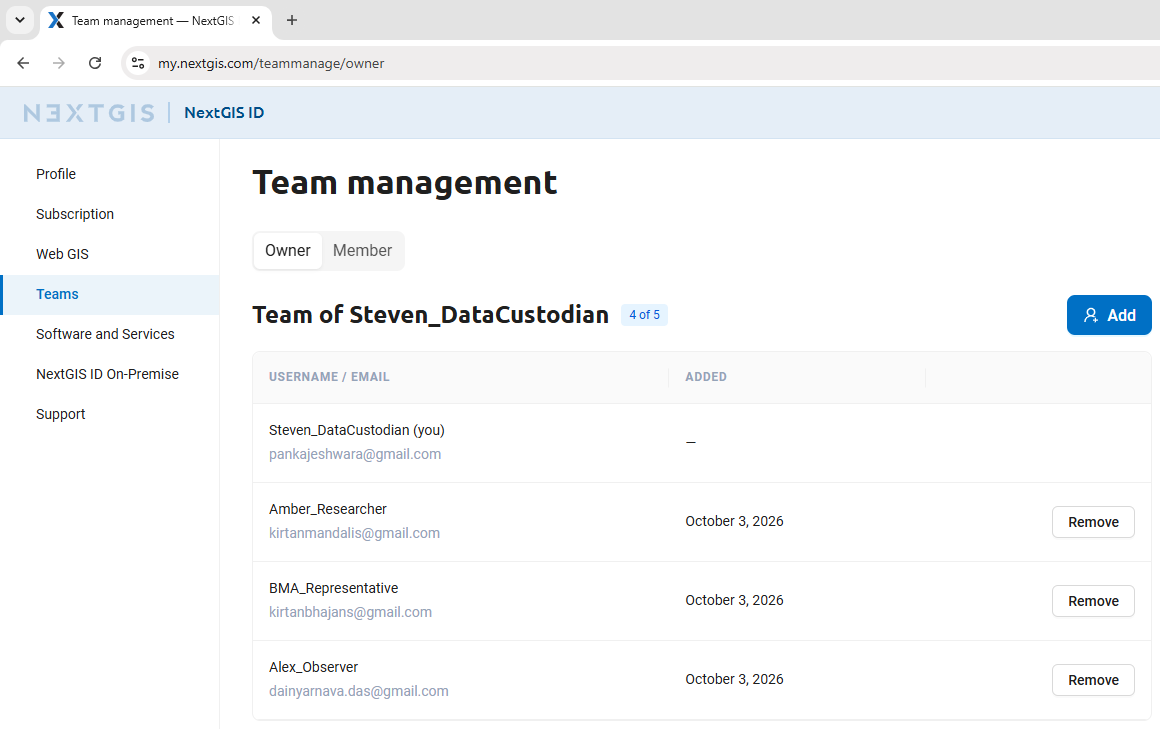
\includegraphics[width=115mm]{nextgis-web.png}
%	\caption{The NextGIS ID team used for the MapSafe Community~A evaluation. The four participating accounts are identified by their case-study roles: Steven--Data Custodian, Amber--Researcher, BMA Representative, and External Test User. Team membership establishes the collaboration context, while access to public keys, anonymised layers, and encrypted packages is controlled separately through Web GIS resource ACLs and OpenPGP recipient selection.}
%	\label{fig:nextgis-community-team}
%\end{figure}

NextGIS administration is intentionally separated from field operation. Before fieldwork, an authorised administrator creates or selects the Web GIS, configures \textit{NextGIS} ID/team membership, creates the relevant authentication group, and applies resource \textit{access-control lists} (ACLs) \citep{nextgis2026users,nextgis2026permissions}. Figure~\ref{fig:nextgis-community-team} shows the four accounts prepared for the Community~A evaluation: \textit{Steven--Data Custodian, Amber--Researcher, BMA Representative,} and \textit{External Test User}. These descriptive profile names identify their roles in the case study; they do not themselves grant access to community resources. Team membership establishes the collaboration context, while the Web GIS group and resource ACLs determine which anonymised layers or encrypted packages each account can discover and download. Access to the plaintext inside an encrypted package additionally requires the user's public key to have been selected during \textit{OpenPGP} encryption. Invitation acceptance, account recovery, compromised-account response, membership removal, and storage administration are best completed through the \textit{NextGIS} Web browser interface. In the field, \textit{MapSafe Mobile} consumes an existing authenticated account and group; group creation remains available only when the signed-in account has the necessary server permission.

Thus, the first community connection is normally prepared in \textit{NextGIS} Web rather than created entirely inside MapSafe. The mobile application reuses the authenticated NextGIS account, lets the user select an existing group, publishes only the user's public key, synchronises accepted member keys, and exchanges the resources permitted by the configured ACLs. MapSafe can create an authentication group for an account with the required server permission, but this convenience action starts with the current user and does not replace browser-based member invitations or resource-permission administration.

\begin{figure}[h!]
	\centering
	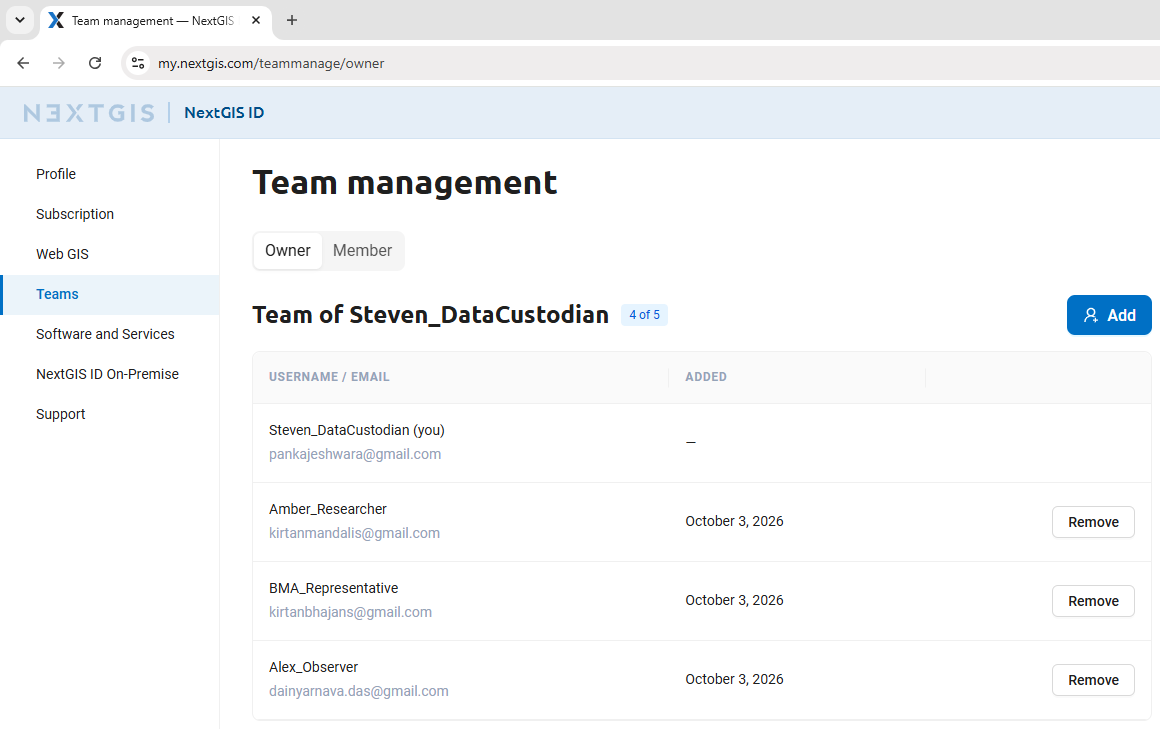
\includegraphics[width=\linewidth]{nextgis-web.png}
	\caption{The NextGIS ID team prepared for the four-account MapSafe Community~A evaluation. The displayed names indicate the participants' case-study roles; access to community resources remains governed separately by Web GIS ACLs and OpenPGP recipient selection.}
	\label{fig:nextgis-community-team}
\end{figure}

\FloatBarrier
\subsection{Encryption identity, key custody, and community public-key exchange}
\label{sec:key-management}

Each participant creates one persistent local OpenPGP identity. Steven supplies a name, organisation, optional email address, and recovery passphrase of at least 12 characters. MapSafe generates an RSA-3072 primary key for certification and signing and a separate RSA-3072 encryption subkey. The transferable secret keyring is protected by an iterated-and-salted SHA-256 string-to-key process, and the application-private copy is additionally encrypted with AES-GCM under a non-exportable \textit{Android Keystore} key. The recovery passphrase is not stored. On later application starts the repository checks the application-private identity store; if a valid identity exists, the encryption screen displays it and does not ask Steven to create another one.

Only public-key material is distributed. A private key is unlocked in memory only for signing or decryption and is never uploaded through the \textit{NextGIS} exchange. Steven, participating BMA representatives, and Amber may each explicitly export their own passphrase-protected secret-key backup before device loss, reset, or application removal. Such backups should be retained on encrypted removable media in a controlled location, with the passphrase held separately by its owner. An end-to-end encrypted channel is preferable if a backup must be transferred remotely. \textit{MapSafe Mobile} cannot recover a forgotten passphrase.

In \emph{Security \& Sharing}, Steven selects an authenticated \textit{NextGIS} account and authentication group representing the relevant community. \textit{MapSafe Mobile} creates or uses the group-scoped directory \path{mapsafe_keys_<group-id>}. Each member publishes a member-owned bucket containing \path{public-key.asc} and \path{key-metadata.json}. Publishing code rejects private-key and passphrase material. The same synchronisation operation is exposed through \emph{Refresh community keys} on the settings and encryption screens.

Discovery is not proof of identity. The client checks current group membership, bucket ownership and uniqueness, manifest/group agreement, agreement between the manifest and downloaded OpenPGP fingerprint, and availability of a usable encryption subkey. The BMA representative's discovered key remains ineligible until Steven compares its full fingerprint through an independent trusted channel and explicitly accepts it. Acceptance pins the fingerprint locally. Changed, missing, duplicate, revoked, or removed-member keys are quarantined and cannot be selected for new packages. Accepted keys are cached for offline use, although membership and key changes require later connectivity. Removing a member prevents selection for future packages but cannot withdraw access to a package already encrypted for that member's key \citep{wouters2024openpgp}.

\begin{figure*}[h!]
  \centering
  \begin{subfigure}[t]{0.31\textwidth}
    \includegraphics[width=\linewidth]{\mapsafefigdir/ms2026-north-whangarei-20260909-18-identity-creation-filled.png}
    \caption{Identity and passphrase.}
  \end{subfigure}\hfill
  \begin{subfigure}[t]{0.31\textwidth}
    \includegraphics[width=\linewidth]{\mapsafefigdir/ms2026-north-whangarei-20260909-19-identity-created.png}
    \caption{Key ID and fingerprint.}
  \end{subfigure}\hfill
  \begin{subfigure}[t]{0.31\textwidth}
    \includegraphics[width=\linewidth]{\mapsafepremiumfigdir/ms2026-premium-community-20261004-00-steven-security-community-keys.png}
    \caption{Live community key directory.}
  \end{subfigure}
  % The broader Security & Sharing screen is retained for possible later use:
  % \begin{subfigure}[t]{0.235\textwidth}
  %   \includegraphics[width=\linewidth]{\mapsafefigdir/ms2026-north-whangarei-20260909-03-security-identity-folder-network.png}
  %   \caption{Public-key exchange, save folder, and network configuration.}
  % \end{subfigure}
  \caption{Persistent identity and group-scoped public-key exchange. Steven creates a locally protected identity, reviews its fingerprint, and synchronises the published keys of \textit{Amber} and the BMA representative from Community A.}
  \label{fig:mapsafe-key-exchange}
\end{figure*}

\FloatBarrier
\subsection{Geospatial anonymisation and derived-layer sharing}
\label{sec:anonymisation}

% MapSafe offers halo masking and hexagonal binning as alternative derived representations. Neither overwrites the authoritative source. Halo masking retains one feature and its non-spatial attributes for each input point but replaces its coordinate. For input point $p_i=(\lambda_i,\phi_i)$, a cryptographically secure random generator selects a bearing uniformly from $[0,2\pi)$ and a displacement within the user-selected interval $[r_{\min},r_{\max}]$. The destination is calculated on a sphere of radius 6,371,000~m rather than by adding planar degree offsets. The compact mobile screen uses one dual-ended range slider for the minimum and maximum distance.

% After each candidate is generated, MapSafe calculates Spruill's disclosure-risk measure. A candidate contributes to risk when its corresponding source point is the nearest member of the original point set. Nearest-neighbour search uses a three-dimensional unit-sphere $k$-d tree, with equal-distance ties containing the parent counted as parent-nearest. For $n$ pairs,
% \begin{equation}
%  R_{\mathrm{Spruill}}=\frac{100}{n}\sum_{i=1}^{n} I_i,
%  \qquad
%  P_{\mathrm{inv}}=100-R_{\mathrm{Spruill}},
%  \label{eq:spruill}
% \end{equation}
% where $I_i=1$ when the source corresponding to masked point $i$ is its nearest original point, and $I_i=0$ otherwise. The interface displays the inverted score so a higher value communicates lower parent-nearest disclosure risk. The result card is collapsible so the map and candidate remain visible. \emph{Remask} returns to the controls but always starts from the precise source, preventing compounded displacement.

As the first safeguarding step, \textit{MapSafe Mobile} allows a field data custodian to create a less precise representation for people who need to understand the general spatial pattern but are not authorised to receive exact locations. \textit{Steven} begins with the 23-point \textit{North Whangārei} dataset, chooses \emph{Halo Masking}, and sets the minimum and maximum displacement on one dual-ended range slider (Figure~\ref{fig:mapsafe-anonymisation}a). \textit{MapSafe Mobile} then creates a new masked layer while leaving the authoritative source unchanged. The case-study attributes and one-to-one relationship between records are retained, but each coordinate is replaced by an approximate location that \textit{Steven} can compare with the source on the unobstructed map (Figure~\ref{fig:mapsafe-anonymisation}b) before sharing it with an authorised community recipient.

\begin{figure*}[h!]
  \centering

  \begin{subfigure}[t]{0.31\textwidth}
    \includegraphics[width=\linewidth]
      {\mapsafefigdir/ms2026-north-whangarei-20260909-10-halo-masking-configuration.png}
    \caption{Dual-ended minimum and maximum displacement control.}
  \end{subfigure}\hfill
  %
  \begin{subfigure}[t]{0.31\textwidth}
    \includegraphics[width=\linewidth]
      {\mapsafefigdir/ms2026-north-whangarei-20260909-29-original-and-halo-masked-unobstructed.png}
    \caption{Original and halo-masked point layers with the result card collapsed.}
  \end{subfigure}\hfill
  %
  \begin{subfigure}[t]{0.31\textwidth}
    \includegraphics[width=\linewidth]
      {\mapsafefigdir/ms2026-north-whangarei-20260909-11-halo-masking-applied-expanded.png}
    \caption{Expanded result with the inverted Spruill score and workflow actions.}
  \end{subfigure}

  \caption{MapSafe Mobile halo-masking workflow for the North Whangārei dataset. Steven sets a displacement interval, compares the original and transformed points on an unobstructed map, and expands the result card when the score or next actions are required.}
  \label{fig:mapsafe-anonymisation}
\end{figure*}


The native Kotlin implementation follows the donut-masking approach demonstrated by \emph{MaskMy.xyz} \citep{swanlund2020maskmy}. For each input point $p_i=(\lambda_i,\phi_i)$, a cryptographically secure random generator selects a bearing uniformly from $[0,2\pi)$ and a displacement within the chosen interval $[r_{\min},r_{\max}]$. 
%The destination is calculated on a sphere of radius 6,371,000~m rather than by adding planar degree offsets. 
The minimum distance moves the candidate away from its precise source, whereas the maximum distance limits the accompanying loss of spatial utility. Figure~\ref{fig:mapsafe-anonymisation}b overlays the original red points and resulting blue masked points for visual comparison while the collapsed result card leaves most of the mobile map unobstructed.

Protecting privacy generally favours greater displacement, while preserving analytical usefulness favours smaller displacement. To help \textit{Steven} balance these competing aims, \textit{MapSafe Mobile} automatically calculates \textit{Spruill's} disclosure-risk measure after each masking attempt \citep{armstrong1999geographically,swanlund2020maskmy}. A transformed point contributes to disclosure risk when its corresponding source point remains the nearest member of the original point set.
% For $n$ original--masked pairs,
% \begin{equation}
%  R_{\mathrm{Spruill}}=\frac{100}{n}\sum_{i=1}^{n} I_i,
%  \qquad
%  P_{\mathrm{inv}}=100-R_{\mathrm{Spruill}},
%  \label{eq:spruill}
% \end{equation}
%where $I_i=1$ when the source corresponding to masked point $i$ is its nearest original point, and $I_i=0$ otherwise. Nearest neighbours are found using a three-dimensional unit-sphere $k$-d tree; an equal-distance tie that contains the parent is conservatively counted as parent-nearest.
The interface reports the inverted value, $P_{\mathrm{inv}}$, so that a higher score communicates a lower parent-nearest disclosure risk and is easier for a field data guardian to interpret (Figure~\ref{fig:mapsafe-anonymisation}c). The score is guidance rather than a guarantee of anonymity, because disclosure also depends on local geography, attributes, auxiliary information, and the intended use.

After reviewing the result, \textit{Steven} may collapse the information card to expose almost the entire map, save the layer locally, upload it for an authorised community recipient through the selected \textit{NextGIS} community, stop the safeguard process, or continue to encryption. If the displayed privacy--utility balance is unsuitable, \emph{Remask} returns to the same controls and generates another candidate. Remasking always begins with the precise source rather than the already displaced layer, preventing offsets from being compounded unintentionally.

The physical-device measurements in Table~\ref{tab:performance-results} distinguish the fast numerical masking calculation from the complete workflow experienced by the guardian. For the 1,000-point typical dataset, coordinate displacement required a median of 35.72~ms, displacement plus Spruill assessment required 120.73~ms, and the complete production workflow required 5.71~s. The corresponding rich-profile medians were 35.79~ms, 120.87~ms, and 5.96~s. At 2,000 points, the typical and rich complete-workflow medians were 10.81 and 11.52~s respectively. Source reading and output-layer writing, rather than the displacement formula, therefore dominate the mobile operation.

The earlier browser and QGIS studies remain useful contextual comparisons, but their shapefile conversion, nesting, implementation language, hardware, and timing boundaries differ from the present Android experiment. The mobile values are therefore reported from the production NextGIS workflow rather than interpreted as a direct speed-up or slowdown relative to JavaScript in a browser or Python in \textit{QGIS}. This scope distinction also avoids attributing storage and layer-management costs to \textit{Spruill's} nearest-neighbour calculation itself.

% Hexagonal binning removes the individual-point representation. Points are assigned to cells at a selected resolution, records sharing a cell identifier are grouped, and one polygon with a count attribute is written for each occupied cell. ARM and ARM64 builds use H3 4.1.1. Because the x86/x86\_64 emulator cannot load the packaged H3 native library, it uses a portable Web Mercator hexagonal grid whose resolution-dependent sizes approximate the choices exposed by the interface. The result card is also collapsible and provides \emph{Bin Again}, \emph{Save Layer}, \emph{Stop}, and \emph{Next: Encrypt} actions.


\emph{Hexagonal Binning} is the second anonymisation option in \textit{MapSafe Mobile}. It is intended for situations in which a recipient needs to understand the distribution or concentration of observations but does not require a separate approximate location for every record. Rather than moving each point, MapSafe assigns the original observations to hexagonal cells at a resolution chosen by the data owner. Points sharing the same cell are replaced by one polygon carrying a \texttt{point\_count} attribute. The resulting layer therefore communicates where observations are concentrated while withholding their exact coordinates. The current interface displays the generated cells as translucent blue polygons; the stored count can also support density-based analysis or styling.

\begin{figure*}[h!]
  \centering
  \begin{subfigure}[t]{0.31\textwidth}
    \includegraphics[width=\linewidth]{\mapsafehexbinfigdir/ms2026-north-whangarei-hexbin-20261006-01-configuration-source-only.png}
    \caption{Resolution 6 selected for the original points; the displayed 3.2~km text is the legacy H3~3.x estimate.}
  \end{subfigure}\hfill
  \begin{subfigure}[t]{0.31\textwidth}
    \includegraphics[width=\linewidth]{\mapsafehexbinfigdir/ms2026-north-whangarei-hexbin-20261006-02-applied-source-and-cells.png}
    \caption{Twenty-three points grouped into 16 cells.}
  \end{subfigure}\hfill
  \begin{subfigure}[t]{0.31\textwidth}
    \includegraphics[width=\linewidth]{\mapsafehexbinfigdir/ms2026-north-whangarei-hexbin-20261006-03-collapsed-cells-only.png}
    \caption{Collapsed view of the aggregate polygons only.}
  \end{subfigure}\hfill
  % \begin{subfigure}[t]{0.24\textwidth}
  %   \includegraphics[width=\linewidth]{figures/ms2026-16-hexagonal-binning-applied-collapsed.png}
  %   \caption{Collapsed hexbin result and map.}
  % \end{subfigure}
  \caption{MapSafe Mobile hexagonal-binning workflow for the North Whangārei dataset. Steven selects a resolution level, compares the original observations with the occupied cells, and collapses the result card to inspect the anonymised polygon layer without the earlier halo-masked points.}
  \label{fig:mapsafe-hexagonal-binning}
\end{figure*}

Choosing the resolution requires the same kind of privacy--utility judgement as choosing masking distances. Lower H3 resolutions produce larger cells, grouping observations across a wider area and concealing more positional detail, but they may be too coarse for local analysis. Higher resolutions produce smaller cells and preserve more geographic detail, but can create a sparse surface or cells containing only one observation, which may provide little meaningful protection \citep{rao2021privacy}. The appropriate level therefore depends on the geographic extent, clustering, sensitivity, and intended use of the dataset rather than on a universal default. In the illustrated \textit{North Whangārei} example, Steven selects resolution~6, which in H3~4.x has an average hexagon edge length of approximately 3.72~km and an average cell area of approximately 36.13~km$^2$ \citep{h3cellstats2026}. MapSafe groups the 23 observations into 16 occupied cells, after which Steven compares the source and aggregate layers and inspects the cells without point overlays (Figure~\ref{fig:mapsafe-hexagonal-binning}).

On supported ARM and ARM64 devices, MapSafe performs the indexing with H3 Java 4.1.1 \citep{sahr2003geodesic,uber2018h3}. The x86/x86\_64 emulator used for the screenshots cannot load the packaged H3 native library, so it uses a portable Web Mercator hexagonal grid with resolution-dependent sizes approximating those presented by the interface. Each run creates one binned layer at the selected resolution while leaving the authoritative point layer unchanged. If a different balance is needed for the intended community purpose, \emph{Bin Again} returns Steven to the resolution control and creates another candidate from the precise source. Steven can then save the selected layer, upload it to the chosen NextGIS community, stop the safeguard process, or continue to encryption. The result card can be collapsed so that most of the screen remains available for comparing the aggregation with its geographic context.

\textit{MapSafe Mobile} supports two levels of data sharing: the original dataset and an anonymised representation. Access is determined by the recipient’s role and intended use rather than by fixed categories such as ``trusted'', ``semi-trusted'', or ``untrusted''. A recipient authorised to work with precise locations may receive the original dataset through multi-recipient \textit{OpenPGP} encryption. A recipient who requires only general spatial patterns receives an anonymised representation created using either halo masking or hexagonal binning. Community membership does not automatically grant access to precise locations; the sovereign data owner remains responsible for selecting the appropriate anonymisation method and parameters, choosing the recipients, and ensuring that each representation is suitable for its intended purpose.







Accepted masked and binned layers can remain on the map, be saved as files, or be uploaded to the selected \textit{NextGIS} community as native vector resources. Local outputs use the fixed public folder \texttt{Downloads/MapSafe}; compact feedback shows only the saved filename and an \emph{Open Folder} action. This avoids repeatedly presenting a destination picker in the field. Sharing a derived layer without encryption is an intentional option, but the interface warns that spatial anonymisation reduces risk rather than guaranteeing safety. Attributes, filenames, photographs, timestamps, or small cell counts may still disclose sensitive information \citep{kessler2018geoprivacy,cassa2008re,zimmerman2008quantifying}.

% \FloatBarrier
% \subsection{Original-dataset encryption and multi-recipient OpenPGP}
% \label{sec:encryption}

% Following anonymisation, the encryption screen selects the original source dataset by default rather than the masked or binned candidate. This implements the business rule that the authoritative dataset is the object normally requiring recipient-specific confidentiality. A compact \emph{Choose} action permits a different file when required, and direct entry to encryption is supported without first performing masking or binning.

% When a local identity exists, its public key is checked as a self-recipient by default, allowing the sender to recover the package later. The user may uncheck it, select one or more accepted community recipients, or use both self and community recipients. Creating an identity returns the user to recipient selection and does not initiate encryption automatically. Encryption may therefore address only the sender, only other recipients, or both.

% The implementation uses standard OpenPGP hybrid encryption. A fresh random AES-256 content-encryption key encrypts the compressed dataset once using the RFC~9580 version-2 Symmetrically Encrypted Integrity Protected Data profile and AES-256-GCM. Each selected recipient's RSA encryption subkey encrypts that same content key into a separate public-key encrypted session-key packet. Adding a recipient adds a small key envelope rather than another encrypted copy of the dataset. The binary \texttt{.pgp} file contains the encrypted payload and all recipient envelopes; there is no separate session-key file. If signing is selected, the local passphrase unlocks the signing key in memory and a SHA-256 OpenPGP signature is embedded. Decryption remains compatible with the earlier AES-256/OpenPGP-MDC MapSafe profile.

% \begin{figure*}[t]
%   \centering
%   \begin{subfigure}[t]{0.31\textwidth}
%     \includegraphics[width=\linewidth]{figures/ms2026-20-encrypt-protect.png}
%     \caption{Original selected by default.}
%   \end{subfigure}\hfill
%   \begin{subfigure}[t]{0.31\textwidth}
%     \includegraphics[width=\linewidth]{figures/ms2026-21-recipient-selection.png}
%     \caption{Self and community recipients.}
%   \end{subfigure}\hfill
%   \begin{subfigure}[t]{0.31\textwidth}
%     \includegraphics[width=\linewidth]{figures/ms2026-22-encryption-success.png}
%     \caption{Protected package saved.}
%   \end{subfigure}
%   \caption{Multi-recipient encryption. The dataset is encrypted once with an AES session key, which is independently wrapped for every checked OpenPGP public key.}
%   \label{fig:mapsafe-encryption-flow}
% \end{figure*}

% The encrypted package is written automatically to \texttt{Downloads/MapSafe}; after encryption, the result card appears below the recipient action, followed by \emph{Stop} and \emph{Next: Notarise}. The user may reselect recipients and create a new package. No filesystem destination is requested for each run.

% \FloatBarrier
% \subsection{NextGIS community resources and encrypted-package exchange}
% \label{sec:community-packages}

% MapSafe uses different NextGIS resources for different artefacts. Public keys use the dedicated group-scoped key directory. Masked and hexagonally binned results may be uploaded as ordinary vector resources so authorised members can view them through the Web GIS. Encrypted \texttt{.pgp} packages are opaque files and are stored as attachments to a small publisher-owned vector registry. Each registry entry records an opaque package identifier, SHA-256 digest, publisher and group identifiers, creation time, status, and reserved blockchain metadata. The attachment is assigned an opaque UUID-based filename; the original dataset filename and geographic content are not disclosed in the registry.

% On the sender's device, \emph{Upload to Community} associates the package with the selected account and group. On a recipient's device, the first Access screen lists \emph{Community datasets} in addition to \emph{Encrypted file on this device}. Selecting a community package downloads the attachment to \texttt{Downloads/MapSafe}, recalculates SHA-256, and compares it with the digest in the NextGIS registry before passing it to the integrity screen. A mismatch is rejected. Access remains subject to the Web GIS resource ACLs prepared by the administrator; MapSafe does not infer that every authenticated NextGIS user may read every community package.

\FloatBarrier
\subsection{Dataset selection and multi-recipient OpenPGP encryption}
\label{sec:encryption}

Within this two-level model, the original and anonymised representations remain separate artefacts rather than being placed inside a nested, multi-level encrypted volume. In the running example, \textit{Steven} protects the precise \textit{North Whangārei} observations for himself and the authorised BMA representative, while the halo-masked and hexagonally binned layers are released to Amber under separate community permissions. MapSafe encrypts every selected artefact separately, producing one \texttt{.pgp} package per dataset; it does not combine several representations inside one package. When several datasets are selected, recipient review is repeated for each package so \textit{Steven} can deliberately apply the same or different recipient set. The \emph{Encrypt} activity can be opened after anonymisation or directly from the Safeguard tab, and its compact \emph{Choose} action lets \textit{Steven} review or change the current dataset before recipient selection (Figure~\ref{fig:mapsafe-encryption-flow}a).

\begin{figure*}[h!]
  \centering

  \begin{subfigure}[t]{0.31\textwidth}
    \centering
    \includegraphics[width=\linewidth]
      {\mapsafefigdir/ms2026-north-whangarei-20260909-20-encrypt-protect.png}
    \caption{Selected North Whangārei dataset and persistent local identity.}
    \label{fig:encrypt-protect}
  \end{subfigure}\hfill
  %
  \begin{subfigure}[t]{0.31\textwidth}
    \centering
    \includegraphics[width=\linewidth]
      {\mapsafefigdir/ms2026-north-whangarei-20260909-21-recipient-selection.png}
    \caption{Selection of self and authorised community recipients.}
    \label{fig:recipient-selection}
  \end{subfigure}\hfill
  %
  \begin{subfigure}[t]{0.31\textwidth}
    \centering
    \includegraphics[width=\linewidth]
      {\mapsafefigdir/ms2026-north-whangarei-20260909-22-encryption-success.png}
    \caption{Protected package saved with continuation actions.}
    \label{fig:encryption-success}
  \end{subfigure}

  \caption{MapSafe Mobile multi-recipient encryption workflow. Each selected dataset is
  	encrypted once, which is independently wrapped for
  	every selected OpenPGP public key. The same accepted recipients define the
  	default NextGIS access permissions for the uploaded encrypted package, while
  	OpenPGP controls decryption. If several datasets are selected, each becomes a
  separate protected package.}
  \label{fig:mapsafe-encryption-flow}
\end{figure*}

\textit{Steven} next chooses exactly who should be able to recover the package. If his persistent local identity is available, \textit{MapSafe} selects \textit{Steven's} public key as a self-recipient by default so that he can decrypt the package later. For the tested release, Steven retains that selection and adds the independently verified public key of the BMA representative (Figure~\ref{fig:mapsafe-encryption-flow}b); Amber is deliberately not selected for the encrypted original. The same mechanism can address other authorised recipients in a different release, but recipient selection remains explicit for every package. If \textit{Steven} must create an encryption identity at this point, MapSafe returns to recipient selection afterwards rather than beginning encryption automatically.

After the recipients have been confirmed, \textit{MapSafe} uses standard \textit{OpenPGP} hybrid encryption to create one \texttt{.pgp} package. The application compresses the selected dataset, generates a fresh random AES-256 content-encryption key, and encrypts the dataset once using the RFC~9580 version-2 Symmetrically Encrypted Integrity Protected Data profile and AES-256-GCM \citep{wouters2024openpgp}. It then encrypts that same content key separately with each selected recipient's RSA encryption subkey. These public-key encrypted session-key envelopes and the encrypted payload are stored together inside the single package. Adding another recipient therefore adds a small key envelope rather than another encrypted copy of the dataset. The same accepted community members are assigned the package's NextGIS ACL,
which controls discovery and download, while OpenPGP controls decryption.

This design removes the need to distribute a shared symmetric key or a common dataset passphrase. Each recipient uses their own private key to recover their copy of the session key, while their personal passphrase is used only to unlock that private key locally. Neither the private key nor its passphrase is added to the package or uploaded to NextGIS. If signing is enabled, the owner's passphrase temporarily unlocks the local signing key and MapSafe embeds a SHA-256 OpenPGP signature, allowing recipients to distinguish confidentiality from evidence about the sender. New packages use the AES-256-GCM profile, while decryption remains compatible with the earlier AES-256/OpenPGP-MDC MapSafe profile.


%During encryption, Steven selects his own and the authorised community
%recipients. This selection has two linked effects for the encrypted package:
%each selected public key receives an OpenPGP-wrapped session key, and the same
%accepted community members are granted permission to discover and download the
%uploaded package. The two controls therefore use one user decision while
%retaining their distinct technical roles: OpenPGP determines who can decrypt,
%whereas NextGIS permissions determine who can access the package resource.




Table~\ref{tab:performance-results} is the mobile equivalent of the masking, encryption, and decryption tables reported for the earlier browser and QGIS versions of MapSafe. The primary datasets contain 50, 250, 500, and 1,000 points because these sizes reflect observations likely to be collected during a NextGIS Mobile field session; 2,000-point datasets provide an additional stress case. Every point-count class has two GeoJSON attribute profiles. Both contain the same 18-field typed schema, but the \emph{rich} profile uses longer, non-repeating notes and stewardship text and is approximately four times larger than the corresponding \emph{typical} file. Attachments are excluded because the current MapSafe GeoJSON exporter does not embed NextGIS attachments.

%The performance experiment was conducted on the physical Samsung handset summarised in Table~\ref{tab:performance-device}. Ten synthetic GeoJSON datasets represented five point counts---50, 250, 500, 1,000, and 2,000---under typical and rich attribute profiles. For every dataset, the test harness evaluated the complete halo-masking workflow, signed OpenPGP encryption, and verified OpenPGP decryption, producing 30 dataset--operation cells. Their execution order was randomised using the fixed seed 20260811. Each cell was completed once as an unreported warm-up and then five times for measurement. Table~\ref{tab:performance-results} reports the median of these five measurements to two decimal places; the corresponding first and third quartiles are retained in the archived result files. Halo masking used fixed 100--2,000~m displacement bounds. The OpenPGP tests used one RSA-3072 identity generated before measurement, one selected recipient, signing enabled, compression, AES-256-GCM encryption, integrity checking, and signature verification.
%
%\begin{table}[t]
%\centering
%\caption{Main specifications of the physical handset used for the MapSafe Mobile performance experiment.}
%\label{tab:performance-device}
%\small
%\begin{tabularx}{\linewidth}{p{0.34\linewidth}X}
%\toprule
%\textbf{Item} & \textbf{Configuration} \\
%\midrule
%Handset & Samsung Galaxy A14 (SM-A145F; product \texttt{a14nsxx}) \\
%System-on-chip & Samsung Exynos 850; eight logical processors \\
%Usable system memory & 3,863,203,840 bytes (approximately 3.60~GiB; 4~GB class) \\
%\bottomrule
%\end{tabularx}
%\end{table}

The performance experiment was conducted on a physical Samsung Galaxy A14 (SM-A145F; product \texttt{a14nsxx}) equipped with a Samsung Exynos 850 system-on-chip, eight logical processors, and approximately 3.60~GiB of usable memory (4~GB class). Ten synthetic GeoJSON datasets represented five point counts---50, 250, 500, 1,000, and 2,000---under typical and rich attribute profiles. For every dataset, the test harness evaluated the complete halo-masking workflow, signed OpenPGP encryption, and verified OpenPGP decryption, producing 30 dataset--operation cells. Their execution order was randomised using the fixed seed 20260811. Each cell was completed once as an unreported warm-up and then five times for measurement. Table~\ref{tab:performance-results} reports the median of these five measurements to two decimal places; the corresponding first and third quartiles are retained in the archived result files. Halo masking used fixed 100--2,000~m displacement bounds. The OpenPGP tests used one RSA-3072 identity generated before measurement, one selected recipient, signing enabled, compression, AES-256-GCM encryption, integrity checking, and signature verification.

The three masking columns deliberately use different boundaries. \emph{Mask core} records source-coordinate normalisation, cryptographically secure displacement, and spherical destination calculation. \emph{Core+SM} includes Spruill's nearest-neighbour assessment on that same candidate. \emph{Complete mask} begins when the already selected NextGIS source layer is read and ends after output-feature construction, transactional insertion, spatial-index rebuilding, and map saving. The cryptographic cells exercise the same production OpenPGP engine over in-memory byte streams. Encryption starts with prepared WGS84 GeoJSON bytes and ends when the signed single-recipient package bytes have been produced; decryption includes private-key unlocking, payload recovery, integrity checking, and signature verification and ends when the plaintext bytes have been recovered. Android file-picker interaction and filesystem input/output are not part of these two cryptographic timings. Human interaction, initial dataset import, UI rendering, community transfer, blockchain access, and result-log writing are also excluded. Hexagonal binning was not timed in this experiment and must be evaluated separately on the physical H3 implementation.

\begin{table*}[t]
\centering
\caption{Median MapSafe Mobile processing times on the Samsung SM-A145F after one warm-up and five measured repetitions.}
\label{tab:performance-results}
\small
\setlength{\tabcolsep}{2pt}
\begin{tabular*}{\textwidth}{@{\extracolsep{\fill}}llrrrrrrr@{}}
\toprule
\textbf{Points} & \textbf{Profile} & \multicolumn{1}{c}{\textbf{Input}} & \multicolumn{3}{c}{\textbf{Masking}} & \multicolumn{2}{c}{\textbf{OpenPGP}} & \multicolumn{1}{c}{\textbf{Output}} \\
\cmidrule(lr){3-3}\cmidrule(lr){4-6}\cmidrule(lr){7-8}\cmidrule(lr){9-9}
& & \textbf{KiB} & \begin{tabular}[c]{@{}c@{}}\textbf{Core}\\\textbf{(ms)}\end{tabular} & \begin{tabular}[c]{@{}c@{}}\textbf{Core+SM}\\\textbf{(ms)}\end{tabular} & \begin{tabular}[c]{@{}c@{}}\textbf{Complete}\\\textbf{(s)}\end{tabular} & \begin{tabular}[c]{@{}c@{}}\textbf{Encrypt}\\\textbf{(s)}\end{tabular} & \begin{tabular}[c]{@{}c@{}}\textbf{Decrypt}\\\textbf{(s)}\end{tabular} & \begin{tabular}[c]{@{}c@{}}\textbf{PGP}\\\textbf{KiB}\end{tabular} \\
\midrule
50    & Typical & 39.76    & 1.90 & 5.35 & 0.32 & 2.34 & 2.32 & 15.12 \\
50    & Rich    & 163.20   & 1.81 & 4.11 & 0.32 & 2.42 & 2.38 & 111.34 \\
250   & Typical & 198.98   & 12.61 & 78.33 & 1.75 & 2.41 & 2.36 & 67.74 \\
250   & Rich    & 816.16   & 8.97 & 21.40 & 1.43 & 2.80 & 2.63 & 550.12 \\
500   & Typical & 398.12   & 17.61 & 46.76 & 2.87 & 2.49 & 2.42 & 133.53 \\
500   & Rich    & 1,632.49 & 16.35 & 41.99 & 2.79 & 3.36 & 2.93 & 1,098.60 \\
1,000$^{\dagger}$ & Typical & 796.39   & 35.72 & 120.73 & 5.71 & 2.68 & 2.52 & 265.18 \\
1,000 & Rich    & 3,265.13 & 35.79 & 120.87 & 5.96 & 4.24 & 3.52 & 2,195.48 \\
2,000 & Typical & 1,594.87 & 65.04 & 180.31 & 10.81 & 3.06 & 2.73 & 528.41 \\
2,000 & Rich    & 6,532.37 & 70.06 & 200.23 & 11.52 & 6.14 & 4.69 & 4,389.20 \\
\bottomrule
\end{tabular*}
\end{table*}

\noindent Each timing is reported to two decimal places. Milliseconds are retained for the two numerical masking phases because expressing them to hundredths of a second would obscure their differences; complete masking, encryption, and decryption are shown in seconds. Encryption and decryption concern one dataset in one single-recipient package rather than nested representation levels, and the 2,000-point rows are stress cases. Because every cryptographic run used one recipient, the results do not quantify the time or package-size overhead of adding recipients. The 1,000-point typical masking median marked $^{\dagger}$ comes from a verification repeat after transient device contention affected three repetitions in the complete run; its cryptographic medians remain from the complete run.

Only one encryption and one decryption column are required because \textit{MapSafe Mobile} does not repeatedly encrypt nested fine, medium, and coarse representations. The anonymised output remains a separate shareable layer, while the original dataset is encrypted once for the selected recipients. For 50 points, the typical and rich profiles each completed the masking workflow in a median of 0.32~s. At 1,000 points, the typical profile required 5.71~s and the rich profile 5.96~s. The similar values at a fixed point count, despite the rich input being approximately four times larger, show that feature count and \textit{NextGIS} layer I/O influence complete masking more strongly than exported GeoJSON byte size. For the 1,000-point rich dataset, coordinate displacement itself required a median of 35.79~ms and displacement plus Spruill assessment required 120.87~ms. These calculation times are small compared with the 5.96~s complete workflow because reading, constructing, inserting, indexing, and saving the derived layer dominate the operation experienced by the guardian.

Signed encryption and verified decryption showed a fixed cryptographic and stream-processing cost for small inputs and then increased with GeoJSON byte size. The 50-point typical dataset required median times of 2.34~s for encryption and 2.32~s for decryption. At 1,000 points, the typical dataset required 2.68~s and 2.52~s respectively, whereas the larger rich dataset required 4.24~s and 3.52~s. The 2,000-point rich stress file (6.38~MiB) required 6.14~s for encryption and 4.69~s for decryption, corresponding to median throughputs of 1.04 and 1.36~MiB/s. The 1,000-point rich dataset reached 0.75~MiB/s for encryption and 0.91~MiB/s for decryption. Compression made every \texttt{.pgp} package smaller than its GeoJSON input. The archived quartiles show generally modest variability, but they are omitted from the compact table in favour of one median per cell. Repeating the initially contended 1,000-point typical masking cell produced a complete-workflow median of 5.71~s, which is the masking value reported in Table~\ref{tab:performance-results}.

These \textit{Android} values should not be compared directly with the throughput reported for the earlier browser and QGIS implementations. The mobile experiment includes the production NextGIS read/write path and signed OpenPGP processing, uses different input formats and hardware, and tests field-scale rather than national datasets. The 1,000-point rich dataset provides a useful upper reference for the intended field workflow: its median complete-masking, encryption, and decryption times were 5.96, 4.24, and 3.52~s respectively. The longest measured median was 11.52~s for complete masking of the 2,000-point rich stress dataset. Raw measurements, phase timings, dataset hashes, device metadata, and both the complete and verification runs are archived with the OSF package (https://osf.io/cyfu7). %source repository at commit \texttt{6edcbb27a03ba76eea78915f097a877969d733d4}.\footnote{\url{https://github.com/sharmapn/nextgis_mobile_mapsafe_geoprivacy/}}

The completed package is written automatically to \texttt{Downloads/MapSafe}, and the result card confirms the saved filename (Figure~\ref{fig:mapsafe-encryption-flow}c). The owner may stop at this point, continue to notarisation, upload the package to the selected NextGIS community, or reselect recipients and create a new package. The package payload remains opaque to \textit{NextGIS} because the service does not possess an addressed private key; the package filename and descriptive registry metadata remain visible to authorised community members and should therefore avoid sensitive wording. Encryption and decryption performance for the intended 50--1,000-point mobile datasets is reported in Table~\ref{tab:performance-results}; unlike the earlier nested scheme, the measured processing time increases principally with dataset size.

\FloatBarrier
\subsection{NextGIS community resources and protected-resource exchange}
\label{sec:community-packages}

\textit{MapSafe} uses different \textit{NextGIS} resources for different artefacts. Public keys use a dedicated group-scoped key directory. Halo-masked and hexagonally binned results are uploaded as native vector resources so authorised members can view or reuse them through the Web GIS. Encrypted \texttt{.pgp} packages remain opaque attachments associated with a publisher-owned package registry. A registry entry records the package filename, SHA-256 digest, publisher and group identifiers, creation time, status, and available blockchain metadata. \textit{MapSafe} never offers an unencrypted original dataset through this upload workflow.

Steven opens \emph{Upload to Community} from the Safeguard tab and may select a public key, one or more anonymised datasets, one or more encrypted packages, or any combination of these items (Figure~\ref{fig:mapsafe-community-exchange}a). Each selection is published under his authenticated account and currently selected group. On the BMA representative's device, \emph{Community Packages} lists the recipient-restricted protected original together with any anonymised layers permitted by its ACL (Figure~\ref{fig:mapsafe-community-exchange}b). Amber sees the community's halo-masked and hexagonally aggregated datasets but is not offered the encrypted original because her key was not selected for that package (Figure~\ref{fig:mapsafe-community-exchange}c). Public keys can be synchronised for later recipient selection, anonymised layers can be downloaded as GeoJSON, and authorised protected packages can be downloaded to \texttt{Downloads/MapSafe} for verification and decryption.

\begin{figure*}[t]
  \centering
  \captionsetup{width=0.96\textwidth}
  \begin{subfigure}[t]{0.30\linewidth}
    \captionsetup{width=\linewidth,justification=centering}
    \includegraphics[width=\linewidth]{\mapsafepremiumfigdir/ms2026-premium-community-20261004-01-steven-upload-community-four-selected.png}
    \caption{Steven selects items to publish.}
  \end{subfigure}\hfill
  \begin{subfigure}[t]{0.30\linewidth}
    \captionsetup{width=\linewidth,justification=centering}
    \includegraphics[width=\linewidth]{\mapsafebmafigdir/ms2026-premium-community-20261006-07-bma-community-package-selection.png}
    \caption{The BMA representative receives the protected original.}
  \end{subfigure}\hfill
  \begin{subfigure}[t]{0.30\linewidth}
    \captionsetup{width=\linewidth,justification=centering}
    \includegraphics[width=\linewidth]{\mapsafebmafigdir/ms2026-premium-community-20261006-05-amber-anonymised-community-access.png}
    \caption{Amber receives anonymised layers only.}
  \end{subfigure}
  \caption{Observed Premium community exchange for the North Whang\={a}rei case. Steven publishes selected resources; the BMA representative receives the recipient-encrypted original, whereas Amber's view contains only the authorised anonymised layers.}
  \label{fig:mapsafe-community-exchange}
\end{figure*}

% Earlier single-account Web GIS transport screenshots are excluded because the
% live Premium multi-account evidence above supplies the manuscript's
% community-exchange figure.
\iffalse
\begin{figure*}[t]
  \ContinuedFloat
  \centering
  \begin{subfigure}[t]{0.45\textwidth}
    \includegraphics[width=\linewidth,trim=0 320 300 0,clip]{\mapsafewebfigdir/nextgis-community-public-keys.png}
    \caption{Community public-key registry.}
  \end{subfigure}\hfill
  \begin{subfigure}[t]{0.45\textwidth}
    \includegraphics[width=\linewidth,trim=0 320 300 0,clip]{\mapsafewebfigdir/nextgis-community-encrypted-packages.png}
    \caption{Publisher-owned package registry.}
  \end{subfigure}
  \par\medskip
  \begin{subfigure}[t]{0.70\textwidth}
    \includegraphics[width=\linewidth,trim=0 180 300 0,clip]{\mapsafewebfigdir/nextgis-community-anonymised-datasets.png}
    \caption{Halo-masked and hexagonally aggregated resources.}
  \end{subfigure}
  \caption{Archived single-account Web GIS transport evidence.}
  \label{fig:mapsafe-nextgis-live-community}
\end{figure*}
\fi

 A four-account Premium acceptance test was executed against the live North Whang\={a}rei community. It published \textit{Steven's}, \textit{Amber's}, and the \textit{BMA representative's} public-key records, two anonymised layers, and one original dataset encrypted and signed for Steven and the BMA representative. As shown in Figure~\ref{fig:nextgis-community}, these resources are organised within separate \textit{Public Keys}, \textit{Anonymised Datasets}, and \textit{Encrypted Packages} groups under MapSafe Community~A. Steven and the BMA representative downloaded byte-identical copies of the protected package; the BMA representative recovered a byte-identical copy of the original and verified Steven's signature. Amber could list and download the two anonymised layers but could neither list nor directly read the protected package, while the external test user could not discover or directly read any Community~A resource. Wrong-key and wrong-passphrase attempts produced no plaintext.

When an encrypted community package is selected, \textit{MapSafe} downloads it, recalculates its SHA-256 digest, and compares the result with the digest recorded in the NextGIS registry before passing the package to the integrity screen; a mismatch is rejected. Access to the resource hierarchy shown in Figure~\ref{fig:nextgis-community} remains subject to the Web GIS ACLs configured by the administrator. Group membership identifies the relevant community, but MapSafe does not infer that every authenticated NextGIS user may read every resource; access is determined separately for public keys, anonymised datasets, and recipient-restricted encrypted packages.

\begin{figure}[h!]
	\centering
	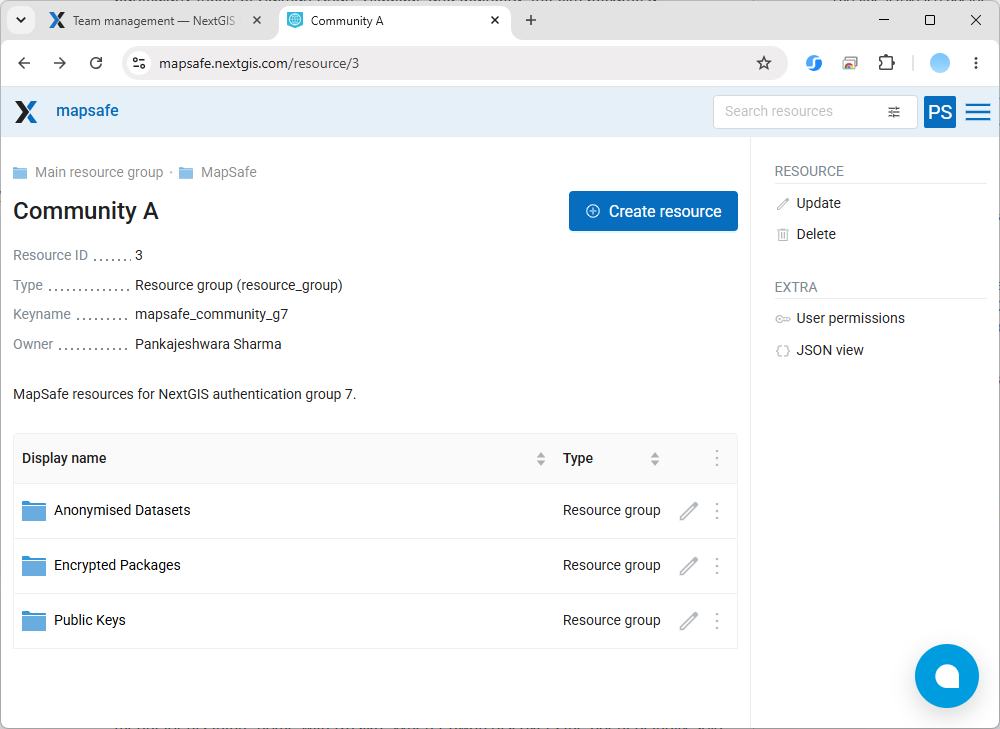
\includegraphics[width=\linewidth]{nextgis-web_details.png}
	\caption{The MapSafe Community~A resource structure in NextGIS Web. Separate resource groups organise community members' OpenPGP public keys, anonymised datasets, and encrypted packages. Access to these resources is governed by Web GIS ACLs associated with the corresponding NextGIS authentication group.}
	\label{fig:nextgis-community}
\end{figure}

\subsection{Notarisation and blockchain-verification boundary}
\label{sec:notarisation}

The \textit{Notarise} screen automatically receives the encrypted package created by the preceding step and calculates its SHA-256 digest. If \textit{Steven} opens it independently, he can select an existing encrypted package. Only the active network name is shown on the operational screen. Network details are configured in \emph{Security \& Sharing}, where \textit{MapSafe} stores encrypted app-private profiles for Ethereum Sepolia, Ethereum Mainnet, or a custom EVM-compatible network. Preflight checks validate the RPC chain identifier, deployed bytecode, expected \texttt{mintNFT(string)} and \texttt{locations(uint256)} selectors, and ERC-721 interface support before the profile is used.

For a new notarisation, \textit{MapSafe} normalises the encrypted package basename and appends an underscore followed by its 64-character lowercase SHA-256 digest. This filename--digest string is encoded as the argument to \texttt{mintNFT(string)}. Binding the public package name to the digest gives the resulting assertion more evidential context than a hash alone: the signing wallet asserted that the named encrypted package had those bytes at the transaction time. It does not expose the plaintext dataset or cryptographic secrets, and it cannot by itself prove the human identity controlling the wallet, prevent another transaction from recording a competing assertion, or make a user-selected filename an intrinsic property of the bytes. Neutral encrypted-package names should therefore be used where a descriptive name would itself disclose sensitive information.

\textit{MapSafe} constructs a zero-value transaction and hands it through Reown WalletConnect to an installed external wallet, such as \textit{Trust Wallet} or \textit{MetaMask}, for explicit review, fee approval, and signing \citep{reown2026walletkit}. The application neither collects nor stores the blockchain private key or recovery phrase. After submission, \textit{MapSafe} retrieves the receipt, verifies that the call was mined successfully on the configured chain and contract, and compares the decoded filename and digest with the local package before reporting success. The transaction hash and network can then be associated with the corresponding community package. This function is complementary to \textit{OpenPGP}: the blockchain record supplies an independently retrievable public assertion about the protected package, while recipient encryption and the optional OpenPGP signature establish confidentiality, package integrity, and signer status.

Network and contract details, including RPC and contract preflight checks, remain in \emph{Security \& Sharing}; the operational Notarise screen carries forward the encrypted filename, calculates its digest, displays the active network and connected wallet, and requests external-wallet approval. Figure~\ref{fig:mapsafe-notarisation} shows the available configuration, contract-checking, and wallet-handoff screens. The Verification screen shown in Figure~\ref{fig:mapsafe-access-flow}b also accepts a transaction reference and, when one is supplied, performs the local-to-chain filename and digest comparison.

\begin{figure*}[h!]
  \centering
  \begin{subfigure}[t]{0.31\textwidth}
    \centering
    \includegraphics[width=\linewidth]{\mapsafefigdir/ms2026-north-whangarei-20260909-04-blockchain-network-profile.png}
    \caption{Active EVM network profile.}
  \end{subfigure}\hfill
  \begin{subfigure}[t]{0.31\textwidth}
    \centering
    \includegraphics[width=\linewidth]{\mapsafefigdir/ms2026-north-whangarei-20260909-05-blockchain-contract-validation.png}
    \caption{Contract and RPC preflight controls.}
  \end{subfigure}\hfill
  \begin{subfigure}[t]{0.31\textwidth}
    \centering
    \includegraphics[width=\linewidth]{\mapsafefigdir/ms2026-north-whangarei-20260909-23-notarisation-hash-network.png}
    \caption{Filename--digest record and wallet hand-off.}
  \end{subfigure}
  \caption{MapSafe Mobile's notarisation workflow. Steven selects an EVM network profile, validates the configured RPC endpoint and contract, and prepares a filename--SHA-256 assertion for approval and signing in an external wallet. These screens document configuration and transaction preparation; external-wallet approval and mined-transaction confirmation occur subsequently.}
  \label{fig:mapsafe-notarisation}
\end{figure*}

\FloatBarrier
\subsection{Verification, decryption, and map display}
\label{sec:verification}

Access begins either from the community package list or the Android file picker. In the tested release, the BMA representative opens \emph{Community Packages} and can discover the encrypted original because the package registry ACL includes that account; Amber can discover only the authorised anonymised layers. Selecting \emph{Download \& verify} saves the \texttt{.pgp} file to \texttt{Downloads/MapSafe}, calculates SHA-256, and compares the downloaded bytes with the digest recorded in the NextGIS registry. A mismatch is rejected before the package reaches the decryption stage.

\begin{figure}[!t]
  \centering
  \begin{subfigure}[t]{0.31\textwidth}
    \captionsetup{font=small,justification=centering}
    \includegraphics[width=\linewidth]{\mapsafebmafigdir/ms2026-premium-community-20261006-07-bma-community-package-selection.png}
    \caption{The BMA representative discovers the protected original.}
  \end{subfigure}\hfill
  \begin{subfigure}[t]{0.31\textwidth}
    \captionsetup{font=small,justification=centering}
    \includegraphics[width=\linewidth]{\mapsafebmafigdir/ms2026-premium-community-20261006-08-bma-package-verification.png}
    \caption{Downloaded bytes are hashed and checked against the community record.}
  \end{subfigure}\hfill
  \begin{subfigure}[t]{0.31\textwidth}
    \captionsetup{font=small,justification=centering}
    \includegraphics[width=\linewidth]{\mapsafebmafigdir/ms2026-premium-community-20261006-09-bma-private-key-decryption.png}
    \caption{MapSafe locates the addressed BMA private key.}
  \end{subfigure}\hfill
%  \begin{subfigure}[t]{0.235\textwidth}
%    \captionsetup{font=small,justification=centering}
%    \includegraphics[width=\linewidth]{\mapsafebmafigdir/ms2026-premium-community-20261006-11-bma-decrypted-original-map.png}
%    \caption{The recovered original is displayed directly on the map.}
%  \end{subfigure}
  \caption{Recipient-side access to the protected original. The BMA representative discovers and downloads the authorised community package, verifies its recorded digest, unlocks the matching local OpenPGP private key, and would later display the recovered North Whang\={a}rei dataset after the earlier map layers are cleared.}
  \label{fig:mapsafe-access-flow}
\end{figure}

The Verification screen can additionally accept a compatible blockchain transaction URL or hash. When one is supplied, MapSafe retrieves the transaction and receipt, checks the configured chain, contract, call, and receipt status, strictly decodes the record, and compares both the normalised encrypted filename and digest. Earlier hash-only MapSafe records remain readable but establish only a digest match. This blockchain comparison is optional for a package that was not notarised; the community-package evidence in Figure~\ref{fig:mapsafe-access-flow}b therefore shows the completed local and registry check before decryption, while the optional transaction field remains available.

The package contains one encrypted dataset. MapSafe inspects its OpenPGP recipient identifiers and locates the BMA representative's matching local secret encryption key (Figure~\ref{fig:mapsafe-access-flow}c). The representative's personal passphrase unlocks that private key in memory, the key recovers the AES session key from its recipient envelope, and the session key decrypts the payload. The session key is therefore an internal cryptographic value rather than a second file that the recipient must manage. A package addressed only to another recipient is rejected, as confirmed by the wrong-key test.

AEAD/MDC integrity and signature authenticity are evaluated separately. Modified or structurally invalid packages are rejected before plaintext is accepted, while a present signature is reported as valid, invalid, or made by an unknown signer. In the four-account acceptance test, the BMA representative recovered a byte-identical GeoJSON copy and MapSafe verified Steven's signature. The result is saved to \texttt{Downloads/MapSafe}, imported as one local NextGIS vector layer, selected, and zoomed to its extent. Previously loaded layers are cleared before display, so the access workflow proceeds directly to the recovered North Whang\={a}rei original rather than opening an intermediate dataset catalogue (Figure~\ref{fig:mapsafe-access-flow}d).
\FloatBarrier

% The earlier commented evaluation template contained unfilled result markers and duplicate tables.
% It is omitted from this illustrative preview because measured performance is reported above,
% while the constructed effectiveness protocol and results are reported below.


%\section{Usability-Informed Design Verification and Illustrative Effectiveness Scenario}
%\label{sec:usability-design}
%
%The MapSafe Mobile's key feature is its interface’s simplicity and documentation. The
%interface is relatively clean, and the masking, hexagonal binning, encryption, notarisation, verification, and decryption aspects themselves have explanatory tooltips next to almost every button. The original, masked and binned datasets are displayed as
%\textit{NextGIS} layers, enabling users to visually explore what the datasets look like before and after anonymising. Moreover, a basic guide to all these aspects is available online (see Section XXXX) to assist new users in understanding how the mobile app works, what the tradeoffs are and how to weigh them, for instance, how to decide on masking distances, as well as some of the app's limitations. The guide also features a video that documents the safeguarding and access process from start to finish. After the user downloads their anonymised dataset or encrypted volumes, additional information is
%displayed to remind them not to reveal specific masking parameters to the
%public, and to safeguard the passphrase used for encryption. After the notarisation,
%the URL address where the encrypted dataset’s details are stored and displayed.
%
%
%\textit{MapSafe Mobile} was designed to make safeguarding decisions understandable at the point of field collection without hiding their consequences. A single workflow panel separates \emph{Safeguard} from \emph{Access} with a two-state tab control, presents the current stage through compact progress indicators, and uses \emph{Stop} and \emph{Next} to let a data custodian end with a useful intermediate artefact or continue. Halo-masking and hexabinning result cards can be collapsed so that the map remains visible, while encryption, verification, and decryption screens show only the information needed for the current decision. The fixed \texttt{Downloads/MapSafe} folder, automatic recognition of an existing encryption identity, explicit dataset selection, community resource lists, and direct display of a recovered layer reduce repeated file selection and unnecessary navigation.
%
%The design was informed by the usability evaluation previously conducted for the \textit{MapSafe QGIS plugin} \citep{sharma2025mapsafe}. That study followed the effectiveness, efficiency, and satisfaction dimensions of ISO~9241-11:2018 \citep{ISO2018ergonomics}. 
%%Its first author observed three professionals---two from GIS and one from cybersecurity, all with academic backgrounds---while they completed safeguarding and access tasks. 
%Satisfaction was examined using Nielsen's heuristic method \citep{nielsen1995conduct}. 
%The evaluated tasks covered geomasking, hexagonal binning, encryption, notarisation, verification, decryption, and display. The accompanying heuristic workbooks and written comments identified issues concerning visible system status, navigation, workflow order, file selection, recognition rather than recall, configuration validation, passphrase visibility, error recovery, screen density, output handling, and contextual help.
%
%These findings were used as formative design evidence rather than being presented as a new participant evaluation of \textit{MapSafe Mobile}. The QGIS tasks and evaluator comments were mapped to the corresponding mobile screen or interaction and classified as \emph{implemented}, \emph{adapted}, \emph{partially addressed}, or \emph{not applicable}. %Generative AI assistance (OpenAI Codex, accessed October 2026) was used to extract and group candidate correspondences across the earlier paper, evaluation workbooks, current interface text, and implementation. 
%Each mapping was then checked against the current source code and recorded workflows. 
%%AI output was not treated as participant evidence, an independent evaluator, a usability score, or a substitute for observed user behaviour. 
%The resulting traceability audit is reported in Appendix Table~\ref{tab:usability-traceability}.
%
%The transfer was appropriate because both implementations use the same principal functional sequence: creating an anonymised representation through masking or hexagonal binning, encrypting selected data, notarising an encrypted artefact, verifying its integrity, decrypting it, and displaying the recovered data. The implementations are not assumed to be identical. \textit{MapSafe Mobile} uses a two-level original/anonymised model, standard multi-recipient \textit{OpenPGP} packages, \textit{NextGIS} community exchange, an external wallet, touch interaction, Android document providers, and substantially smaller screens. %Desktop-specific recommendations concerning resizable windows, minimising a QGIS plugin, keyboard Escape behaviour, and simultaneous interaction with other QGIS tools were therefore not transferred mechanically.
%
%The audit showed that findings directly affecting the critical safeguarding and access path were incorporated into the mobile design. These include visible progress and operation status; consistent \textit{Back}, \textit{Stop}, and \textit{Next} controls; early source-layer checks; deliberate dataset and recipient selection; recognition of an existing identity; return to recipient selection after identity creation; passphrase visibility controls; validation of blockchain profiles; exclusion of unencrypted originals from community upload; and specific \textit{OpenPGP} messages for incorrect passphrases, non-recipient keys, invalid packages, and integrity failures. Other recommendations were adapted to the platform: broad Android document selection is followed by format and content checks rather than relying solely on MIME filtering, and long desktop panels became collapsible mobile result cards. Convenience features such as comprehensive in-application help, one-action cleanup of all derived layers, and copying every displayed digest remain only partially addressed and are identified explicitly rather than being counted as completed usability findings.
%
%This process demonstrates traceability from earlier empirical findings to present design decisions; it does not itself measure \textit{MapSafe Mobile} task-completion rates, interaction time, learnability, satisfaction, or accessibility. The QGIS participants' results are therefore not attributed to the mobile application. Touch input, small displays, Android storage providers, intermittent field connectivity, community-account administration, and external-wallet approval may introduce problems that were absent from the desktop evaluation. An independent mobile study and participatory evaluation with the communities whose authority and information are represented remain necessary before making broader claims about usability or cultural legitimacy.
%
%%\subsection{Illustrative effectiveness protocol}
%
%%To show how a present-day effectiveness evaluation could be reported, this preview models 
%%one GIS professional who is familiar with Android field mapping but has not previously used MapSafe, OpenPGP recipient selection, or external-wallet notarisation. 
%%The evaluator is assumed to use the Samsung Galaxy A14 described in the performance experiment, a prepared NextGIS community containing Steven's, the BMA representative's, and Amber's public keys, a configured external wallet, and the 23-point North Whangārei demonstration dataset. 
%For our effectiveness evaluation, we engaged a GIS professional who is familiar with Android field mapping to complete the 12 safeguarding and access tasks listed in Appendix Tables~\ref{tab:usabilitytasks} and~\ref{tab:illustrative-effectiveness} twice. Each repetition began from the same prepared state so the task sequence is comparable. Effectiveness is represented by task completion, user error, system error, assistance, and recovery. A \emph{critical error} would expose an unencrypted original, irreversibly alter the source, encrypt for the wrong recipient without detection, accept an invalid verification result, or prevent recovery of the intended dataset. A \emph{non-critical error} is a reversible action that is blocked or corrected without compromising the source or protected package.
%
%%The values below are deliberately hypothetical. They are not observations made by a participant and are included only to preview the analysis, appendix structure, and claims that could follow from an actual evaluation. The scenario assumes that 
%
%The evaluator initially tries to continue before accepting the BMA representative's public-key fingerprint, waits in MapSafe instead of moving to the external wallet for transaction approval, and enters an incorrect private-key passphrase once. The first and third events are corrected from MapSafe's messages without assistance; the wallet transition requires one short moderator prompt. No corresponding error is modelled in the second repetition.
%
%%\subsection{Illustrative effectiveness results}
%
%Under this scenario, all 24 task trials---12 tasks across two repetitions---are completed, giving an illustrative completion rate of 100\%. Twenty-one trials are error-free (87.50\%). The first repetition contains three non-critical user errors and therefore nine error-free tasks out of 12 (75.00\%); the second contains no user errors and all 12 tasks are error-free. No system errors, critical errors, source modifications, unintended plaintext uploads, incorrect-recipient encryptions, false integrity acceptances, or unrecovered datasets are modelled. Two of the three first-repetition errors are recovered through the interface without assistance. One assistance event is required for external-wallet hand-off, equivalent to 4.17\% of the 24 task trials. The detailed task-level account appears in Appendix Table~\ref{tab:illustrative-effectiveness}; Appendix Table~\ref{tab:usabilitytasks} presents the same scenario in the compact format used by the earlier MapSafe evaluation.
%
%If observed in a real study, these results would indicate strong effectiveness for the central protection path: every intended artefact is produced or recovered, and the interface prevents the evaluator's mistakes from becoming security failures. The disappearance of errors in the second repetition would also provide preliminary evidence of short-term learnability. The scenario nevertheless identifies the external-wallet transition as the most likely interruption and supports adding contextual guidance at that point. It does not test satisfaction, accessibility, long-term retention, unfamiliar Android document providers, poor connectivity, malicious inputs, or community administration, and a single evaluator would be insufficient for population-level usability claims.


\section{Usability-Informed Design and Evaluation}
\label{sec:usability-design}

The principal usability objective of \textit{MapSafe Mobile} is to make safeguarding and access decisions understandable during field collection. The interface separates \emph{Safeguard} and \emph{Access}, shows progress and consistent \emph{Back}, \emph{Stop}, and \emph{Next} actions, keeps masking and binning results visible through collapsible cards, recognises existing identities and community keys, and displays the recovered layer directly after decryption. These choices reduce repeated navigation while keeping the consequences of each operation visible.

The evaluation approach was adapted from the earlier \textit{MapSafe QGIS plugin} study \citep{sharma2025mapsafe} and follows the effectiveness, efficiency, and satisfaction dimensions of ISO~9241-11:2018 \citep{ISO2018ergonomics}. The evidence is deliberately distinguished: effectiveness was tested through the mobile workflow, efficiency was assessed using physical-device measurements, and the earlier interface findings were used as formative design evidence. Mobile-user satisfaction was not measured.

For \textit{effectiveness}, the first author completed the 12 safeguarding and access tasks listed in Appendix Table~\ref{tab:usabilitytasks}, twice from the same prepared North Whang\={a}rei and Community~A state. All 24 trials were completed successfully, giving a 100\% task-completion rate. No user or system errors, critical errors, assistance events, unintended plaintext uploads, incorrect-recipient encryptions, false integrity acceptances, or unrecovered datasets were recorded. The authoritative layer remained unchanged, derived layers were created separately, and the community workflow did not offer an unencrypted original for publication. This demonstrates functional effectiveness under prepared conditions, not independent first-time-user usability.

For \textit{efficiency}, the physical-device measurements in Table~\ref{tab:performance-results} show that the principal local operations are practical for field-scale datasets. The 1,000-point rich dataset required median times of 5.96~s for complete masking, 4.24~s for signed encryption, and 3.52~s for verified decryption. Notarisation was excluded from the fixed processing time because wallet approval, transaction submission, connectivity, and blockchain confirmation are external and variable.

\textit{Formative interface evidence} came from the QGIS study's heuristic inspection and comparable safeguarding and access tasks \citep{nielsen1995conduct}. Its recommendations concerning status visibility, navigation, file selection, recognition rather than recall, passphrase handling, screen density, output management, help, and error recovery were mapped to the mobile activities; the resulting traceability audit is provided in Appendix Table~\ref{tab:usability-traceability}. Progress and validation feedback were implemented directly, while large desktop panels were adapted as collapsible mobile cards and file selection was followed by format and content validation. These inherited findings are design evidence, not satisfaction results from mobile participants; independent testing of mobile satisfaction, accessibility, and learnability remains necessary.

%The previous satisfaction results cannot establish satisfaction with the mobile application because touch interaction, small displays, Android document providers, community-account administration, intermittent connectivity, and external-wallet approval introduce different usability conditions. Similarly, the present effectiveness assessment was conducted by an author familiar with the system and was therefore a functional self-evaluation rather than an independent participant study. The results demonstrate that the intended workflow can be completed without observed errors under the prepared test conditions, but independent mobile-user testing and participatory evaluation with the communities whose data and authority are represented remain necessary before making broader claims about usability, accessibility, satisfaction, or cultural legitimacy.

%\section{Discussion}
%\label{sec:discussion}
%
%Sensitive geospatial information is increasingly created on a mobile device, yet privacy and access controls are often applied only after the observation has been synchronised, downloaded, or transferred to a desktop environment. This delay is particularly consequential when the coordinate itself reveals culturally significant places, threatened species, harvesting areas, or other information whose disclosure cannot simply be reversed. MapSafe Mobile addresses this interval by moving representation and access decisions to the device on which the observation is first handled. Its contribution is therefore not merely the transfer of earlier MapSafe functions from a browser or QGIS to Android. It demonstrates how an established mobile GIS workflow can support \emph{capture-time sovereignty}: the ability to apply a legitimate decision about spatial detail, recipients, and integrity evidence before the precise record crosses an external trust boundary.
%
%The two-level sharing model is central to this contribution. MapSafe Mobile treats the original dataset and an anonymised representation as separate artefacts rather than placing several representations inside a nested encrypted volume. A sovereign data owner can share a halo-masked or hexagonally aggregated layer when a recipient requires only general spatial information, while an original or anonymised artefact may also be protected with multi-recipient OpenPGP when recipient-specific confidentiality is required. If several artefacts are selected, MapSafe creates a separate package for each rather than joining them inside one \texttt{.pgp} file. This arrangement avoids treating trust as a universal ranking. A recipient may be a dependable community member but still lack a legitimate reason to receive a precise location. The relevant question is instead which representation and protection are appropriate for the person's role, purpose, and responsibilities. Representation control and cryptographic access control are related, but neither substitutes for the other.
%
%Embedding these functions in NextGIS Mobile also reduces the number of systems through which unprotected data must pass. Halo masking, hexagonal binning, export, encryption, hashing, verification, and decryption are performed locally. Steven can inspect the original or derived layer in its geographic context, save it to a predictable folder, or share the selected artefact through an existing NextGIS community. This integration is important for field practice: a separate specialist application may offer a strong algorithm but still fail operationally if field custodians must export plaintext, understand unfamiliar file conventions, or postpone protection until they return to an office. The open-source implementation additionally permits inspection and adaptation, although source availability alone does not establish that a deployment is secure or governed appropriately.
%
%\subsection{Performance and operational practicality}
%
%The performance evaluation was deliberately centred on datasets containing 50, 250, 500, and 1,000 points. This differs from the large national and archival layers used to assess the earlier browser and desktop implementations, but reflects the intended mobile scenario: a person protects observations collected during a field session. A 2,000-point class was added as a stress case. For the 1,000-point rich dataset, the median complete halo-masking, signed-encryption, and verified-decryption times were 5.96, 4.24, and 3.52~s respectively. For the 2,000-point rich stress dataset, the corresponding medians were 11.52, 6.14, and 4.69~s. All 30 cells in the complete run finished, and the archived quartiles show that the medians were generally stable under the recorded thermal conditions. These results support the operational practicality of local protection for the intended field-session scale on the evaluated handset. They do not measure participant interaction time, learnability, or satisfaction; neither the design traceability review nor the explicitly hypothetical effectiveness scenario in Section~\ref{sec:usability-design} should be interpreted as observed participant evidence.
%
%The results should be interpreted according to the work performed by each operation. Halo displacement is driven mainly by point count, while the production workflow is dominated by reading the source layer and writing and indexing the derived layer. This distinction is empirically important: for the 1,000-point rich dataset, coordinate calculation plus Spruill assessment took a median of 120.87~ms, whereas the complete workflow took 5.96~s. OpenPGP encryption and decryption showed an approximately 2.30-second fixed cost for the smallest files and then increased with the number of exported bytes. The rich attribute profile changed cryptographic time more strongly than masking time at the same point count. Recipient scaling still does not repeat full-payload encryption: the AES-256 content key encrypts the original once, and each additional recipient adds public-key wrapping work and a small session-key envelope. However, because the present experiment used one recipient throughout, it provides no observed recipient-count effect on time or package size; the proposed 1, 2, 5, and 10-recipient experiment remains necessary before making a scaling claim.
%
%Physical-device evaluation is important because processor, storage, memory pressure, Android power management, and thermal behaviour affect field performance. The Samsung SM-A145F remained at Android thermal status~0, and its battery temperature fell slightly from 34.4$^{\circ}$C to 34.1$^{\circ}$C while connected to external power, providing no indication of thermal throttling during the complete run. The benchmark nevertheless used a debug build and the shorter Quick protocol, so it should be treated as preliminary rather than as the final publication run. H3 processing must also be timed separately on ARM or ARM64 hardware; the portable grid used by the x86/x86\_64 emulator is a compatibility fallback rather than an identical benchmark substitute. Network upload, package download, and blockchain retrieval were kept separate from local processing because they depend on connectivity and server conditions. This separation prevents a slow field connection from being presented as a cryptographic limitation, or a fast laboratory connection from obscuring the practical cost of remote exchange.
%
%\subsection{Security and privacy analysis}
%
%The local processing boundary reduces unnecessary disclosure but does not eliminate the need to trust the device. Precise coordinates exist in memory and local storage before transformation, and a compromised operating system, malicious application, insecure backup, screen capture, or retained temporary file could expose them. MapSafe reduces some of this surface by avoiding remote anonymisation and encryption services, deleting temporary exports after use, protecting the application-private secret keyring with Android Keystore encryption, and requiring a passphrase for private-key operations. These measures should complement device encryption, secure updates, controlled backups, and organisational incident-response procedures rather than be treated as replacements for them.
%
%Halo masking offers an understandable privacy--utility control because the minimum distance prevents a transformed point from remaining immediately adjacent to its source and the maximum distance limits loss of geographic usefulness. The inverted Spruill score assists comparison between stochastic candidates. Nevertheless, neither displacement nor a favourable score guarantees anonymity. Re-identification may exploit clustering, road or coastline constraints, attributes, timestamps, photographs, filenames, or external datasets \citep{kessler2018geoprivacy,zhang2022rehumanize,cassa2008re,zimmerman2008quantifying}. Hexagonal binning similarly conceals exact coordinates but may remain revealing when a cell contains a single observation or when a high resolution produces a sparse pattern. MapSafe therefore provides alternative representations and decision support, not a universal privacy certificate.
%
%The OpenPGP design addresses a different problem: who may recover a selected artefact. A fresh AES-256 session key encrypts each dataset once, and that key is independently protected for each selected recipient. The data owner does not need to transmit a shared symmetric key or disclose a common dataset passphrase. Each recipient instead uses a locally held private key and its own passphrase. The sender's key is selected by default as a self-recipient so that the package remains recoverable, while accepted community public keys permit several authorised organisations to receive the same encrypted bytes. Optional signing separates evidence about the sender from encrypted-data integrity. This use of a standard container is preferable to a MapSafe-specific nested format, but interoperability with independent OpenPGP applications remains an important release test.
%
%Public-key encryption shifts rather than removes the identity problem. A mathematically valid public key is not proof that it belongs to the intended person. MapSafe therefore requires fingerprint review before a discovered community key becomes selectable and quarantines changed or inconsistent entries. This limits silent key substitution but introduces a human verification responsibility. Cached accepted keys permit offline field encryption, while delayed synchronisation means that membership changes, revocations, or compromised keys may not be visible until connectivity returns. Removing someone from a NextGIS group prevents their selection for future packages; it cannot withdraw access to a package that was already encrypted for their private key. Key rotation, recovery, revocation, and the handling of device loss consequently remain organisational as well as technical processes \citep{chu2013key,zhang2010wireless,wouters2024openpgp}.
%
%The NextGIS community performs three distinct functions: it identifies the collaboration context, distributes public keys and selected artefacts, and applies server-side resource permissions. These functions should not be conflated. Group membership does not automatically grant access to every resource, so Web GIS ACLs must still be administered. Conversely, permission to download an opaque \texttt{.pgp} attachment does not grant the ability to decrypt it. NextGIS Web can store viewable anonymised layers and encrypted packages without receiving an OpenPGP private key; the upload interface deliberately excludes unencrypted originals. The platform nevertheless remains operationally trusted for account administration, availability, ACL enforcement, and delivery of the current key directory. Community exchange therefore combines server permissions with end-to-end encryption rather than claiming that either mechanism is sufficient alone.
%
%Blockchain evidence has a narrower role. The current record binds a normalised encrypted-package filename to its SHA-256 digest, enabling a verifier to test whether a selected named package is byte-for-byte identical to the artefact asserted by the signing wallet at the transaction time. It cannot establish that the underlying observation was accurate, that collection was authorised, that the selected recipients were legitimate, or that disclosure is ethically acceptable. The current build supports configurable EVM profiles, contract preflight, external-wallet signing and submission, receipt validation, transaction retrieval, and strict filename--digest comparison without storing a wallet key. This is completed technical notarisation in the evaluated research configuration, but it is not trustless proof of authorship or meaning. Production deployment still requires evaluation of contract security, wallet identity, fees, network selection, confirmation depth, recovery, comprehension, and failure handling.
%
%\subsection{Usability-informed design}
%
%Security controls are ineffective when users cannot understand the decisions they are being asked to make. Section~\ref{sec:usability-design} therefore traces the earlier MapSafe QGIS evaluation findings to the current mobile implementation. The transfer provides a documented basis for decisions concerning system status, user control, error prevention, recognition rather than recall, screen density, and recovery messages. It does not provide participant-derived evidence about mobile effectiveness, efficiency, satisfaction, or learnability, and the earlier QGIS completion and error results are not reused as MapSafe Mobile outcomes.
%
%The illustrative two-repetition scenario shows what favourable effectiveness evidence would look like if subsequently observed: all 24 task trials complete, 87.50\% are error-free overall, three reversible user errors occur in the first repetition, none occur in the second, and no critical or system error produces an unsafe outcome. The modelled recipient-key and passphrase mistakes are recovered through interface feedback, while the external-wallet transition accounts for the sole assistance event. This pattern would support the interpretation that validation and recovery controls protect the workflow even when a first-time user makes a mistake, while also identifying wallet hand-off guidance as a specific improvement. Because the values were constructed rather than observed, however, they demonstrate the intended analysis and cannot establish that real users will achieve the same completion or recovery rates.
%
%Several design choices seek to make secure behaviour the natural path. Missing input is reported before spatial parameters are entered. Encryption makes the selected dataset visible, recognises an existing identity automatically, and preselects the owner's key as a recoverable self-recipient. Creating an identity returns to recipient selection instead of silently starting encryption, and unencrypted originals are omitted from community uploads. Collapsible result cards preserve the map as the main visual evidence, while \emph{Stop} and \emph{Next} preserve user control without imposing a compulsory wizard. Verification, private-key unlocking, successful decryption, and map access are presented as separate stages. The predictable save folder removes repeated destination dialogs but also requires a clear retention and cleanup policy.
%
%These choices illustrate why security and usability need not be treated as simple opposites. Error prevention, visible state, familiar map context, and reduced repetition can support stronger behaviour rather than dilute it \citep{nielsen1995conduct}. At the same time, simplifying labels must not obscure consequences. Users still need to understand that anonymisation does not guarantee safety, that accepting a public-key fingerprint is an identity decision, that a passphrase protects a private key rather than the dataset directly, and that successful decryption transfers responsibility for the plaintext to the recipient. Documentation, participatory training, and observation of mobile users remain necessary even when the implementation demonstrably incorporates lessons from a closely related desktop workflow.
%
%\subsection{Limitations and future work}
%
%MapSafe Mobile currently focuses on point-vector data. Lines, polygons, trajectories, raster layers, photographs, sensor streams, and complete NextGIS layer packages raise different representation and metadata problems. Sequential mobility points may reveal routes even when individual observations are displaced, and an attached image may retain EXIF coordinates after its map geometry is protected. Future work should develop explicit attachment and metadata policies and evaluate techniques appropriate to these additional data types rather than applying point masking indiscriminately.
%
%The present anonymisation choices are intentionally understandable but limited. Donut masking does not account for population density, address plausibility, networks, coastlines, or other contextual constraints. Verified-neighbour, location-swapping, adaptive urban--rural, and network-constrained masks may offer stronger protection in some settings, but require auxiliary data and introduce new computation, licensing, availability, and privacy concerns. Hexagonal aggregation would benefit from organisation-defined resolution guidance and, where appropriate, minimum-count policies that warn about or suppress singleton cells. Repeated evaluation is needed to determine whether such safeguards improve decisions without making the field interface unmanageable.
%
%Key management also requires further development. The current application supports one local identity per installation and does not yet provide a complete revocation-certificate, organisational certification, key-rotation, or managed recovery interface. Passphrase-protected secret-key backups must be tested across device replacement and application removal, and interoperability should be verified with tools such as GnuPG and OpenKeychain. Live NextGIS evaluation must exercise several accounts, group changes, ACL isolation, package removal, quota behaviour, offline cache staleness, and compromised-account response on physical devices. A community should not depend on an untested recovery path for access to an irreplaceable encrypted archive.
%
%The implemented external-wallet workflow avoids storing a raw Ethereum private key in application preferences or a text file, but its interaction, transaction fees, chain selection, confirmation depth, failure recovery, and accessibility require broader study. The current filename-bound Sepolia deployment is a research configuration; production use requires an audited and governed contract deployment, pinned contract evidence, appropriate network policy, and testing across supported wallets and failure conditions. Further work should also evaluate energy and network costs across the whole workflow rather than attributing them only to the blockchain. More broadly, performance, usability, and technical correctness do not establish cultural legitimacy. Reusing the North Whangārei coordinates with synthetic demonstration attributes cannot substitute for co-design with the relevant BMAs concerning terminology, acceptable spatial detail, authority, retention, reuse, and accountability \citep{kukutai2016indigenous,lovett2019gooddata,carroll2020care,jennings2023care,reyesgarcia2022}.

%\section{Conclusion}
%\label{sec:conclusion}
%
%MapSafe Mobile demonstrates that geoprivacy and recipient control can be introduced at the point where sensitive spatial observations are first handled. By embedding halo masking, hexagonal aggregation, persistent OpenPGP identities, multi-recipient encryption, community exchange, filename-bound notarisation, verification, and direct post-decryption map access within NextGIS Mobile, the approach reduces the need to move plaintext through separate browser, desktop, or server workflows before it can be safeguarded. The authoritative observation remains unchanged, while the data owner chooses between two explicit representation levels: the original and an anonymised alternative. Either may be encrypted for selected recipients as a separate package, while only anonymised layers and encrypted packages---never an unencrypted original---are offered for community upload.
%
%The implementation also clarifies the different responsibilities of its components. Spatial transformation controls what geographic detail is disclosed; OpenPGP controls which selected keys may recover a package; NextGIS groups and ACLs control discovery and server-side access; and the EVM workflow binds an encrypted filename to a digest for later comparison. Each selected payload is encrypted once, with a small public-key envelope added for every recipient, so no shared dataset passphrase or nested representation volume is required. Private keys remain locally protected, the sharing platform cannot decrypt a correctly addressed package, and transaction approval remains inside an external wallet. The physical-device experiment completed all 30 dataset--operation cells and showed that complete masking, signed encryption, and verified decryption remained within approximately six seconds for the primary 50--1,000-point datasets. The QGIS-to-mobile traceability audit confirms that previously identified workflow issues were considered in the mobile design. The illustrative 100\% task-completion scenario shows how effectiveness could be reported and identifies wallet hand-off as a likely assistance point, but it is not a completed participant study. Recipient-count scaling, multi-account community exchange, offline reconnection, blockchain latency, and participant usability therefore remain distinct evaluation requirements.
%
%These controls do not by themselves produce anonymity, trustworthy data, legitimate authority, or Indigenous Data Sovereignty. Masking and aggregation remain vulnerable to contextual inference; public-key security depends on identity verification, recovery, and revocation; authorised recipients can redistribute plaintext; NextGIS administration remains important for membership and resource permissions; and a successful filename-bound blockchain transaction records a wallet's assertion rather than proving the truth or legitimacy of the underlying observation. Subject to these boundaries, broader physical-device functional and multi-account validation, external OpenPGP interoperability, production contract review, and participatory co-design, MapSafe Mobile provides a practical open-source foundation for protecting sensitive field observations before external synchronisation and for making representation, access, and integrity decisions visible within the mobile GIS workflow.
%
%On the Samsung Galaxy A14, the 1,000-point rich dataset produced median complete-masking, encryption, and decryption times of 5.96, 4.24, and 3.52~s respectively after one warm-up and five measured repetitions. For the 2,000-point rich stress dataset, the corresponding medians were 11.52, 6.14, and 4.69~s. The result demonstrates local computational feasibility. The accompanying illustrative effectiveness scenario predicts complete task recovery and no critical errors across two repetitions, but those constructed values cannot substitute for observation of human participants. Security, offline behaviour, community exchange, recipient scaling, blockchain latency, and participant usability therefore require their own evidence and should not be inferred from runtime or from the transfer of findings from the earlier QGIS study. Current EVM support includes configurable profiles, contract preflight, external-wallet transaction approval and submission, receipt retrieval, and filename--digest comparison. Subject to the stated evidential boundaries and participatory validation, MapSafe Mobile provides a practical foundation for protecting sensitive field observations before external synchronisation.


%\section{Discussion}
%\label{sec:discussion}
%
%Sensitive geospatial information is increasingly created and managed through mobile devices, yet privacy and access controls are often applied only after the data have been synchronised, transferred, or opened in a desktop GIS. This creates an important period in which precise coordinates may leave the collecting device before the data custodian has considered whether they should be shared in their original form. The consequences can be particularly serious for culturally significant places, threatened species, harvesting areas, or other locations whose disclosure cannot be reversed. MapSafe Mobile addresses this problem by integrating geospatial anonymisation, encryption, community sharing, notarisation, verification, and decryption into the existing NextGIS Mobile environment. Its main contribution is therefore \emph{capture-time sovereignty}: enabling representation, recipient, and integrity decisions to be made before sensitive observations cross an external trust boundary.
%
%MapSafe Mobile uses a two-level sharing model consisting of the authoritative original dataset and a separately created anonymised representation. Halo masking and hexagonal binning provide different ways of reducing spatial precision, while OpenPGP controls who can recover a selected dataset. These mechanisms address different questions. Anonymisation determines what geographic detail is disclosed, whereas encryption determines who may access the selected representation. A dependable community member may still have no legitimate need to receive exact coordinates, while a purpose-authorised researcher may require the original. The appropriate release therefore depends on the recipient's role, purpose, and responsibilities rather than on a universal hierarchy of trusted, semi-trusted, and untrusted users.
%
%Unlike the earlier nested MapSafe scheme, the mobile application does not place the original and anonymised datasets inside one multi-level encrypted volume. Each selected dataset is treated as an independent artefact and, if encryption is required, is written to a separate \texttt{.pgp} package. This simplifies recovery and allows Steven to apply different recipients to different representations. It also preserves the distinction between a viewable anonymised NextGIS layer and an opaque encrypted package. Integrating these operations into NextGIS Mobile reduces the need to export an unprotected dataset to a separate specialist application and allows Steven to inspect the transformation in its geographic context before saving or sharing it.
%
%The open-source implementation permits inspection and adaptation and provides a model for incorporating privacy controls into other mobile GIS platforms. However, technical availability alone does not establish that a release is legitimate, culturally safe, or appropriately governed. MapSafe helps communicate and enact a disclosure decision; it does not determine who possesses the authority to make that decision.
%
%\subsection{Performance Analysis}
%
%The performance experiment focused on datasets containing 50, 250, 500, and 1,000 points because these sizes reflect observations likely to be collected during a mobile field session. A 2,000-point class was included as a stress case. Each point-count class contained typical and rich attribute profiles, allowing masking to be considered in relation to feature count and encryption and decryption to be considered in relation to exported file size. The tests were conducted on a Samsung Galaxy A14 rather than an emulator, and each operation was measured five times after one warm-up, with the median reported.
%
%For the 1,000-point rich dataset, complete halo masking, signed OpenPGP encryption, and verified decryption required median times of 5.96, 4.24, and 3.52~s, respectively. The corresponding values for the 2,000-point rich stress dataset were 11.52, 6.14, and 4.69~s. These results indicate that the main safeguarding and access operations can be completed within practical times for the anticipated field-session datasets on a modest Android handset.
%
%The results also show that the operations are affected by different dataset properties. Numerical coordinate displacement and Spruill assessment were comparatively fast, while the complete masking workflow was dominated by reading the selected NextGIS layer, constructing the output layer, inserting the transformed features, rebuilding its spatial index, and saving the map. Masking time consequently increased mainly with feature count and remained similar for typical and rich datasets containing the same number of points. Encryption and decryption were more sensitive to file size because the rich profile contained substantially more attribute data. A fixed OpenPGP and stream-processing cost was visible for small inputs, after which processing time increased with the number of bytes.
%
%The encrypted packages were smaller than their GeoJSON inputs because MapSafe compresses the dataset before encryption. This reduction should not be interpreted as an effect of encryption itself, since encrypted content is not inherently smaller. The present experiment used one recipient for each measured package. Adding recipients does not encrypt the complete dataset again: the dataset is encrypted once using a random AES-256 session key, and each additional recipient adds another public-key-encrypted copy of that session key. Nevertheless, recipient-count effects on processing time and package size should be measured directly before making a quantitative scaling claim.
%
%The experiment measured local processing separately from community upload, download, blockchain retrieval, and transaction confirmation. These network operations depend on connectivity, server conditions, wallet interaction, transaction fees, and the selected blockchain. Separating them prevents poor field connectivity from being misinterpreted as slow masking or cryptography. Hexagonal-binning performance also requires a separate physical-device experiment because the x86 emulator used for manuscript screenshots employs a portable compatibility grid, whereas supported ARM devices use the native H3 implementation.
%
%\subsection{Security Analysis}
%
%Executing masking, encryption, hashing, verification, and decryption locally reduces unnecessary disclosure to external processing services. Precise observations can be anonymised or encrypted before being uploaded to the selected NextGIS community. However, local processing does not eliminate the need to trust the handset. The original coordinates exist in memory and local storage before protection, and a compromised operating system, malicious application, insecure backup, screen capture, or retained attachment could reveal them. Android Keystore protection, passphrase-protected secret keys, local device encryption, secure updates, controlled backups, and organisational incident-response procedures must therefore operate together.
%
%Halo masking offers an understandable way of balancing privacy and spatial utility. The minimum distance moves a transformed point away from its precise source, while the maximum limits the accompanying loss of geographic usefulness. The inverted Spruill score helps Steven compare stochastic candidates. Nevertheless, neither displacement nor a high score guarantees anonymity. Re-identification may exploit clustering, roads, coastlines, attributes, timestamps, photographs, filenames, or external datasets \citep{kessler2018geoprivacy,zhang2022rehumanize,cassa2008re,zimmerman2008quantifying}. Hexagonal aggregation also conceals exact coordinates but can remain revealing when a cell contains only one observation or when a high H3 resolution produces a sparse surface. MapSafe consequently provides decision support and alternative representations rather than a universal privacy certificate.
%
%OpenPGP addresses recipient-specific confidentiality. MapSafe generates a fresh AES-256 session key for each protected dataset and encrypts the payload once. That session key is then independently protected using every selected recipient's public encryption key. Steven may include his own key as a self-recipient, the BMA representative's accepted key, or other authorised community keys. Each recipient uses a locally held private key and personal passphrase to recover the session key and decrypt the dataset. A shared dataset passphrase does not need to be communicated separately. Optional signing additionally allows the BMA representative to verify that the recovered package was signed using Steven's key.
%
%Public-key encryption shifts rather than eliminates the identity problem. A valid key does not by itself prove that it belongs to the named community member. MapSafe therefore requires fingerprint review before a discovered public key becomes eligible for recipient selection. Changed, duplicated, inconsistent, revoked, or removed-member keys are quarantined. Cached accepted keys support field encryption when connectivity is unavailable, although delayed synchronisation means that later membership or key changes may not be immediately visible. Removing a member prevents selection for future packages but cannot revoke a package that was previously encrypted for that member's private key \citep{chu2013key,zhang2010wireless,wouters2024openpgp}.
%
%The Premium multi-account test demonstrated the complementary roles of OpenPGP and NextGIS resource permissions. Steven published his public key, two anonymised layers, and an original dataset encrypted and signed for Steven and the BMA representative. The BMA representative downloaded a byte-identical package, recovered a byte-identical copy of the original, and verified Steven's signature. Amber could list and download the authorised halo-masked and hexagonally aggregated layers but could neither list nor directly read the protected original in the tested release. The external test user could not discover or directly access the Community~A resources. Wrong-key and wrong-passphrase attempts produced no plaintext.
%
%These results show that NextGIS group membership, Web GIS access-control lists, and OpenPGP recipient selection provide separate layers of control. Group membership identifies the community but does not automatically grant access to every resource. An ACL permits a user to discover or download an artefact, whereas an OpenPGP recipient envelope determines whether that user can recover the protected plaintext. The upload workflow also excludes an unencrypted original. NextGIS Web remains operationally trusted for account administration, resource availability, ACL enforcement, and delivery of the public-key directory, but it does not hold the private keys needed to decrypt a protected package.
%
%Blockchain notarisation has a narrower evidential role. MapSafe records a normalised encrypted-package filename together with its SHA-256 digest. A verifier can therefore determine whether the selected named package is byte-for-byte identical to the package asserted by the signing wallet at the transaction time. Binding the filename to the digest provides more context than recording an unidentified hash alone, but it does not prove that the underlying observations are accurate, that their collection was authorised, or that the wallet controller possessed legitimate authority. The filename is public and should not disclose a sensitive place or subject. External-wallet signing avoids storing a blockchain private key in MapSafe, while production use would still require appropriate network governance, contract review, fee planning, wallet recovery, and failure handling.
%
%\subsection{Usability Analysis}
%
%Security features are useful only when data custodians and recipients can understand and complete the required operations. MapSafe Mobile therefore uses a compact workflow panel, visible progress indicators, consistent navigation controls, early source-layer validation, automatic recognition of an existing identity, deliberate recipient selection, collapsible result cards, predictable output storage, and specific error messages. These features seek to make secure behaviour the natural continuation of the GIS workflow rather than an unrelated technical process.
%
%The effectiveness evaluation was conducted by the first author using the 12 safeguarding and access tasks reported in the Appendix. Each task was performed twice, producing 24 task trials. All trials were completed successfully, and no user error, system error, critical error, unintended plaintext upload, incorrect-recipient encryption, false verification acceptance, unrecovered dataset, or assistance event was recorded. The source layer remained unchanged, the intended derived and encrypted artefacts were produced, and the appropriate accounts recovered only the representations authorised for them.
%
%These results demonstrate functional effectiveness under the prepared test conditions. Because the evaluator was familiar with the application and involved in its development, they should not be interpreted as an independent estimate of usability for first-time users. A broader study may reveal difficulties involving touch interaction, Android document providers, account configuration, intermittent connectivity, fingerprint comparison, or external-wallet approval that were not encountered in the self-evaluation.
%
%Efficiency was informed by the physical-device measurements rather than by asking the evaluator to repeat timings already dominated by masking, layer construction, encryption, decryption, and blockchain processing. The measured results show that the local safeguarding and access operations are practical for the intended field-scale datasets. Interface overhead was limited by carrying the selected dataset between stages, recognising existing identities, using a fixed save folder, and displaying the recovered layer directly.
%
%User-satisfaction findings were borrowed from the earlier usability evaluation of the \textit{MapSafe QGIS plugin} \citep{sharma2025mapsafe}. That evaluation followed ISO~9241-11:2018 \citep{ISO2018ergonomics} and used Nielsen's heuristic method \citep{nielsen1995conduct}. Its participants valued clear visual cues, progress indicators, documentation, and guided safeguarding and access workflows, while identifying issues involving system status, navigation, workflow order, file selection, recognition rather than recall, configuration validation, passphrase handling, screen density, output management, contextual help, and error recovery.
%
%These findings were used as formative design evidence for MapSafe Mobile rather than being presented as satisfaction results from mobile participants. Desktop findings were mapped to the corresponding mobile activity and implemented or adapted where appropriate. Progress indicators and consistent \emph{Back}, \emph{Stop}, and \emph{Next} actions support workflow orientation; passphrase eye controls support error prevention; existing identities and community keys are recognised rather than repeatedly entered; and large desktop panels became collapsible cards that preserve map visibility. These choices illustrate that security and usability need not be treated as opposing objectives. Clear state, recoverable operations, and reduced repetition can encourage stronger security behaviour rather than weaken it \citep{nielsen1995conduct}. An independent satisfaction study remains necessary because the earlier QGIS participants did not evaluate the Android application.
%
%\subsection{Limitations and Future Work}
%
%MapSafe Mobile currently focuses on point-vector datasets. Lines, polygons, trajectories, rasters, photographs, attachments, and sensor streams raise different privacy and metadata concerns. Sequential points can reconstruct a route even when individual observations are displaced, while images may retain coordinates or other identifying information in their metadata. Future work should develop explicit policies for attachments and metadata and evaluate protection techniques appropriate to these additional data types.
%
%The current anonymisation methods are intentionally understandable but limited. Donut masking does not account for roads, coastlines, address plausibility, population density, or other contextual constraints. Verified-neighbour, location-swapping, network-constrained, and adaptive urban--rural techniques may provide stronger protection in some settings, but they require auxiliary data and introduce further computational, licensing, availability, and privacy concerns. Hexagonal binning would also benefit from organisation-defined resolution guidance and optional minimum-count rules that warn about or suppress singleton cells.
%
%Key and community administration require continued testing. The application currently supports one local OpenPGP identity per installation and does not yet provide a complete organisational certification, revocation, rotation, or managed-recovery interface. Passphrase-protected secret-key backups should be tested across device replacement, application removal, and recovery by intended custodians. Interoperability should also be verified with independent OpenPGP tools. Further NextGIS evaluation should examine membership changes, ACL modifications, resource removal, storage quotas, offline-cache staleness, compromised accounts, and recovery after service interruption.
%
%The external-wallet design avoids storing a raw Ethereum private key in application preferences or a text file, but production notarisation requires further evaluation of contract security, transaction fees, network selection, confirmation policy, wallet comprehension, accessibility, and recovery. Energy and network costs should be evaluated across the complete workflow rather than attributed only to the blockchain.
%
%Finally, performance, functional effectiveness, and technical access control do not establish cultural legitimacy. The North Whangārei demonstration uses existing coordinates with synthetic attributes and cannot substitute for co-design with the relevant BMAs. Decisions concerning acceptable spatial detail, recipient authority, retention, reuse, terminology, and accountability must remain with the people and institutions whose interests and knowledge are represented \citep{kukutai2016indigenous,lovett2019gooddata,carroll2020care,jennings2023care,reyesgarcia2022}. MapSafe Mobile supplies technical mechanisms for enacting such decisions, but it cannot confer sovereignty or legitimacy by itself.

\section{Discussion}
\label{sec:discussion}

Sensitive geospatial information is increasingly collected with mobile devices, yet privacy and access controls are often applied only after synchronisation or transfer to another system. This is consequential when precise coordinates identify culturally significant places, threatened species, harvesting areas, or other sensitive information whose disclosure cannot be reversed. MapSafe Mobile addresses this gap by integrating anonymisation, encryption, community sharing, notarisation, verification, and decryption into NextGIS Mobile. Its main implication is \emph{capture-time sovereignty}: the data owner can decide the spatial detail, recipients, and integrity evidence before the original dataset crosses an external trust boundary.

The two-level model keeps the authoritative original separate from an anonymised representation. Halo masking and hexagonal binning determine what geographic detail is disclosed, while OpenPGP determines who can recover a selected dataset. These are independent decisions: a dependable community member may have no legitimate reason to receive precise coordinates, whereas an authorised BMA representative may need them for sovereign oversight. This distinction makes the release decision explicit for Steven, Amber, and the BMA representative rather than reducing their roles to a single trust label. Unlike the earlier nested MapSafe scheme, each selected dataset is protected as its own artefact and, when encrypted, as a separate \texttt{.pgp} package. This lets Steven select recipients for each representation while keeping protection within the established field-data environment.

In terms of \textit{performance analysis}, the physical-device results indicate that the intended field-scale operations are practical on a modest Android handset. For the 1,000-point rich dataset, complete halo masking, signed OpenPGP encryption, and verified decryption required median times of 5.96, 4.24, and 3.52~s; the 2,000-point stress case required 11.52, 6.14, and 4.69~s. Masking time was driven mainly by feature count and the reading, construction, indexing, and saving of the NextGIS layer, whereas cryptographic time increased with exported bytes, particularly for rich attributes. Compression made the resulting encrypted packages smaller than their GeoJSON inputs. Network transfer, wallet interaction, blockchain retrieval, and transaction confirmation were not included because they depend on external conditions.

As for \textit{security analysis}, we found that local processing reduces unnecessary disclosure to remote services, but it does not remove the need to trust the handset: original coordinates exist in memory and local storage before protection. \textit{Android Keystore} protection, passphrase-protected keys, device encryption, secure updates, controlled backups, and incident response are therefore complementary requirements. The same boundary applies to retained attachments, screenshots, metadata, and automatic device backups. Masking and aggregation improve the privacy--utility trade-off but do not guarantee anonymity; clustering, attributes, timestamps, photographs, external datasets, singleton cells, and sparse H3 resolutions may still support re-identification \citep{kessler2018geoprivacy,zhang2022rehumanize,cassa2008re,zimmerman2008quantifying}.

OpenPGP provides recipient-specific confidentiality by encrypting each selected dataset once with a fresh AES-256 session key and wrapping that key for every selected recipient. In the tested release, Steven encrypted and signed the original for himself and the BMA representative, while Amber received only the authorised masked and binned layers. Fingerprint review is still necessary because a public key is not proof of identity; membership changes or compromised keys may also remain hidden in an offline cache until synchronisation resumes \citep{wouters2024openpgp}. The Premium test illustrates the separation of controls: NextGIS ACLs governed discovery and download, OpenPGP recipients governed decryption, and wrong-key or wrong-passphrase attempts produced no plaintext. NextGIS therefore remains trusted for administration, availability, ACL enforcement, and key distribution, but it does not hold the private keys \citep{nextgis2026permissions,wouters2024openpgp}.

Blockchain notarisation has a narrower role than confidentiality or authority. MapSafe records a normalised encrypted-package filename with its SHA-256 digest so that a verifier can establish byte identity for the named package. This does not prove that the observations are accurate, that collection was authorised, or that the wallet controller had legitimate authority. The filename must therefore avoid sensitive information, and production deployment still requires contract review, network and fee policies, wallet recovery, and failure handling.

In terms of \textit{usability analysis}, \textit{MapSafe Mobile} was designed to make secure behaviour a continuation of the field workflow. Progress indicators, consistent \emph{Back}, \emph{Stop}, and \emph{Next} actions, early layer validation, identity recognition, deliberate recipient selection, collapsible result cards, and predictable output storage reduce technical barriers while keeping the consequences of protection visible. Carrying the selected dataset between stages, recognising stored identities, listing community artefacts, and displaying the recovered layer directly also reduce repeated file navigation. In the first-author effectiveness evaluation, the 12 safeguarding and access tasks were each completed twice (24 trials) without user or system errors, incorrect-recipient encryptions, false integrity acceptances, unintended plaintext uploads, or unrecovered datasets. This demonstrates functional effectiveness under prepared conditions, not independent first-time-user usability.

The design was also informed by the earlier evaluation of the \textit{MapSafe QGIS plugin} \citep{sharma2025mapsafe}, which examined effectiveness, efficiency, and satisfaction using ISO~9241-11:2018 \citep{ISO2018ergonomics} and Nielsen's heuristics \citep{nielsen1995conduct}. The mobile implementation adapted its recommendations on status visibility, navigation, file selection, recognition rather than recall, passphrase handling, screen density, output management, help, and error recovery. Desktop panels became collapsible cards, passphrase visibility was added through eye controls, and existing identities and community keys are recognised automatically. An independent satisfaction and accessibility study remains necessary because the earlier participants did not evaluate the Android application.

Our work is not without \textit{limitations and recommendations for future work}. 
Our evidence is bounded by one Samsung Galaxy A14, one recipient per encrypted package, and local timings that excluded network, wallet, and blockchain latency. The effectiveness assessment was conducted by the first author and did not measure independent satisfaction, accessibility, learnability, or retention. Future benchmarking should vary recipient counts, devices, Android versions, and connectivity, including offline reconnection and confirmation delays.

Deployment also needs stronger lifecycle controls. The current implementation supports one local OpenPGP identity per installation but not complete organisational certification, rotation, revocation, or managed recovery. Backup and restoration should be tested across device replacement, application removal, compromised accounts, membership and ACL changes, stale caches, and service interruption, with interoperability checked against independent OpenPGP tools \citep{wouters2024openpgp,nextgis2026permissions}. Production notarisation also requires governed contract deployment, wallet recovery, fee and network policies, confirmation handling, and failure recovery. Future releases should address lines, polygons, trajectories, rasters, attachments, and metadata, while testing context-aware masking, organisation-defined H3 rules, and minimum-count warnings. Independent usability, interoperability, and participatory studies with the relevant BMAs are needed to determine acceptable spatial detail, recipient authority, retention, reuse, terminology, and accountability. MapSafe Mobile provides mechanisms for those decisions; it cannot confer sovereignty or cultural legitimacy by itself \citep{kukutai2016indigenous,lovett2019gooddata,carroll2020care,jennings2023care,reyesgarcia2022}.

\section{Conclusion}
\label{sec:conclusion}

The growing use of mobile GIS for field data collection highlights the need to protect sensitive geospatial information at the point where it is created. \textit{MapSafe Mobile} addresses this challenge by integrating halo masking, hexagonal binning, encryption, community sharing, blockchain-based notarisation, verification, and decryption into NextGIS Mobile. Bringing these functions into the field-data environment allows custodians to decide what spatial detail should be disclosed, who should receive it, and how its integrity can be verified before the original observations are synchronised or transferred elsewhere. This approach advances the concept of \emph{capture-time sovereignty}, in which safeguarding becomes part of data collection rather than an activity postponed until the data reach a desktop computer or external service.

Protecting a dataset introduces an additional step into the mobile GIS workflow, but failing to safeguard precise locations can lead to irreversible disclosure, loss of trust, and diminished community control. \textit{MapSafe Mobile} demonstrates how anonymisation, recipient-based encryption, resource permissions, and integrity evidence can be combined within an accessible workflow without replacing the familiar map-based environment. Its separation of original and anonymised representations enables disclosure to be matched to the recipient's authorised purpose rather than to a fixed hierarchy of trust. Local processing also reduces reliance on third-party services for handling plaintext, while NextGIS community resources support controlled collaboration between custodians, researchers, sovereign parties, and other authorised recipients. As an open-source implementation, \textit{MapSafe Mobile} additionally provides a transparent and adaptable foundation for organisations seeking to incorporate geoprivacy into mobile field practice.

\textit{MapSafe Mobile} does not by itself guarantee anonymity, establish legitimate authority, or confer Indigenous Data Sovereignty. These outcomes depend on governance, identity verification, appropriate anonymisation parameters, key management, recipient responsibilities, and continuing community oversight. Future work should extend the approach to additional geospatial data types, strengthen key recovery and revocation, evaluate alternative masking strategies, assess production blockchain deployments, and conduct independent and participatory evaluations with the communities whose information is represented. By embedding geoprivacy within mobile GIS, \textit{MapSafe Mobile} demonstrates a practical direction for protecting sensitive observations before external synchronisation and for making disclosure and access decisions more visible, accountable, and closely connected to the people responsible for the data.

% For double-anonymised review, omit author names, affiliations,
% acknowledgements, and identifying repository links from the review manuscript.




\section*{Appendix}

\noindent\textbf{Evaluation protocol and interpretation.} The effectiveness evaluation was conducted by the first author, who is familiar with GIS, Android field mapping, and the MapSafe implementation. The evaluator used the prepared North Whang\={a}rei dataset and configured Community~A state, and completed the 12 safeguarding and access tasks in the order shown in Table~\ref{tab:usabilitytasks}. Each task was performed twice from the same prepared state. The record considered task completion, user errors, system errors, assistance, recovery, and preservation of the authoritative source. A critical error would expose an unencrypted original, irreversibly alter the source, encrypt for an unintended recipient without detection, accept an invalid integrity result, or prevent recovery of the intended dataset. A non-critical error would be a reversible action that was blocked or corrected without compromising the source or protected package. The resulting 24 trials are a functional self-evaluation under prepared conditions; they are not an independent participant study and do not provide mobile user-satisfaction, accessibility, or learnability evidence.

\noindent Table~\ref{tab:usability-traceability} records how findings from the earlier MapSafe QGIS evaluation were transferred to MapSafe Mobile. \emph{Implemented} denotes a direct mobile control or behaviour; \emph{adapted} denotes a platform-appropriate response rather than literal reproduction; \emph{partial} identifies a remaining convenience or documentation gap; and \emph{not applicable} identifies a desktop-specific concern. These classifications describe design traceability, not participant outcomes. Table~\ref{tab:usabilitytasks} combines the success requirements with the outcomes recorded during the first-author effectiveness evaluation. All 24 task repetitions were completed without a user error, system error, critical error, or assistance event.

{\footnotesize
\setlength{\tabcolsep}{3pt}
\renewcommand{\arraystretch}{1.1}
\begin{longtable}{@{}p{0.16\linewidth}p{0.22\linewidth}p{0.40\linewidth}p{0.15\linewidth}@{}}
\caption{Traceability from MapSafe QGIS usability findings to MapSafe Mobile design responses.}
\label{tab:usability-traceability}\\
\toprule
\textbf{Heuristic area} & \textbf{Earlier finding} & \textbf{MapSafe Mobile response} & \textbf{Status} \\
\midrule
\endfirsthead
\caption[]{Traceability from MapSafe QGIS usability findings to MapSafe Mobile design responses (continued).}\\
\toprule
\textbf{Heuristic area} & \textbf{Earlier finding} & \textbf{MapSafe Mobile response} & \textbf{Status} \\
\midrule
\endhead
\midrule
\multicolumn{4}{r}{\scriptsize Continued on next page}\\
\endfoot
\bottomrule
\endlastfoot

Visibility of system status & Retain progress bars and provide prompt feedback after actions. & Safeguard and Access step strips expose the current stage; long-running operations show progress and status text; completion panels name the produced or saved artefact. & Implemented \\

User control and navigation & Add Back, Forward, Previous, exit, and cancellation controls, particularly around encryption and decryption. & Activities and dialogs provide Back navigation; \emph{Stop} leaves the workflow; \emph{Next} continues; \emph{Remask} and \emph{Bin Again} repeat reversible anonymisation decisions. Busy cryptographic operations disable conflicting controls. & Adapted \\

Workflow order and error prevention & Explain the order of masking, encryption, and notarisation and why later controls are unavailable until prerequisites are complete. & Compact step indicators show orientation without imposing a compulsory wizard. Safeguard checks for a compatible selected layer at entry, while each feature validates its own prerequisites. Users may begin directly with encryption or verification when appropriate. & Adapted \\

Recognition rather than recall & Carry masked or binned outputs into encryption and avoid making users repeatedly locate prior inputs. & The artefact selector identifies original, halo-masked, hexagonal-binned, encrypted, and public-key items. Workflow transitions carry the selected output forward; an existing identity is recognised; the owner's key is selected by default; community recipients remain explicit. & Implemented \\

File selection and constraints & Prevent unsupported uploads instead of accepting every file without guidance. & Internal selectors expose recognised MapSafe artefacts and community upload excludes unencrypted originals. Broad Android document-provider selection is retained where MIME filtering previously hid valid \texttt{.pgp} files; selected content is subsequently opened and validated with explicit errors. & Adapted \\

Configuration and secret entry & Validate blockchain fields, apply settings without reloading, and permit optional inspection of obscured secret text. & Network name, chain ID, HTTPS RPC and explorer URLs, and contract-address syntax are validated before use. Saved profiles are read by operational screens without plugin reload. Passphrase and confirmation fields provide eye controls. Wallet private keys are never collected by MapSafe. & Implemented \\

Error recognition and recovery & Replace generic decryption errors with causes such as an incorrect passphrase. & OpenPGP failures distinguish an incorrect passphrase, a package not addressed to the device's key, an invalid OpenPGP message, missing integrity protection, a failed integrity check, an unknown signer, and an invalid signature. & Implemented \\

Aesthetic and minimalist design & Preserve a clean interface and avoid controls or explanations that compete with the task and map. & Safeguard and Access share one tabbed launcher; non-functional privacy controls and repeated explanations were removed; the masking range uses one dual-ended control; result cards collapse upward so the map remains visible. & Implemented \\

Output handling and continuity & Use explicit Save labels, simplify destination selection, preserve progress, and make hashes easy to retain. & Outputs use the predictable \texttt{Downloads/MapSafe} folder, show the saved filename, and provide \emph{Open Folder}. Identities and settings persist, while hashes and transaction references are retained with package records. Copy controls are not yet provided for every displayed digest. & Partial \\

Layer management & Provide a quick way to clear multiple trial anonymisation layers. & Successful decryption clears previously loaded layers and displays only the recovered dataset. A single command for removing every earlier halo or hexagonal candidate has not been added. & Partial \\

Help and documentation & Link controls to contextual help and provide a concise overview or FAQ. & Headings, concise decision text, stage indicators, confirmation messages, and the planned workflow video provide guidance, but a searchable in-application FAQ and control-level help links remain future work. & Partial \\

Desktop window behaviour & Fix or minimise the plugin window, confirm closure through Escape, and allow interaction with other QGIS tasks. & MapSafe Mobile uses Android activities and dialogs rather than a resizable desktop plugin window; Android Back, lifecycle restoration, and collapsible map overlays replace these desktop-window behaviours. & Not applicable \\
\end{longtable}
}

\subsection*{Combined effectiveness record}

{\scriptsize
\setlength{\tabcolsep}{2pt}
\renewcommand{\arraystretch}{1.08}
\begin{longtable}{@{}p{0.095\linewidth}p{0.355\linewidth}p{0.06\linewidth}p{0.06\linewidth}p{0.13\linewidth}p{0.25\linewidth}@{}}
\caption{Combined MapSafe Mobile effectiveness task and outcome record from the first-author evaluation. \emph{Rep.~1} and \emph{Rep.~2} report whether the success requirement was met. The error/assistance cell reports user errors and assistance prompts as R1 values followed by R2 values; no system or critical error was recorded.}
\label{tab:usabilitytasks}\\
\toprule
\textbf{Task} & \textbf{Success requirement} & \textbf{R1} & \textbf{R2} & \begin{tabular}[c]{@{}c@{}}\textbf{Errors/}\\\textbf{assist.}\end{tabular} & \textbf{Outcome} \\
\midrule
\endfirsthead
\caption[]{Combined MapSafe Mobile effectiveness task and outcome record (continued).}\\
\toprule
\textbf{Task} & \textbf{Success requirement} & \textbf{R1} & \textbf{R2} & \begin{tabular}[c]{@{}c@{}}\textbf{Errors/}\\\textbf{assist.}\end{tabular} & \textbf{Outcome} \\
\midrule
\endhead
\midrule
\multicolumn{6}{r}{\scriptsize Continued on next page}\\
\endfoot
\bottomrule
\endlastfoot
1. Entry & Stable Safeguard/Access tabs, entry with a compatible point layer, and an immediate understandable warning when spatial input is missing. & Met & Met & 0/0; 0/0 & Early source confirmation prevents a late incompatible-layer failure. \\
2. Halo masking & A separate masked layer, an unchanged authoritative source, a visible inverted Spruill score, and sufficient map space to inspect the candidate. & Met & Met & 0/0; 0/0 & The result and score remain visible while the source is preserved. \\
3. Hexbinning & A count-bearing polygon layer at the selected H3 resolution without overwriting the original points. & Met & Met & 0/0; 0/0 & The aggregate is inspected before safeguarding continues. \\
4. Identity & Matching passphrases supported by visibility controls, no automatic encryption after creation, and recognition of the identity when encryption is reopened. & Met & Met & 0/0; 0/0 & Eye controls support comparison and identity creation returns to recipient selection. \\
5. Recipients & Clear distinction between the self-recipient and community recipients, with full-fingerprint acceptance required before the BMA representative can be selected. & Met & Met & 0/0; 0/0 & The fingerprint requirement prevents an unaccepted community key from being selected. \\
6. Encryption & One package for the original in \texttt{Downloads/MapSafe}, explicit filename confirmation, and recovery by Steven and the BMA representative but not by an unselected identity. & Met & Met & 0/0; 0/0 & The destination is reported and both selected identities recover the package. \\
7. Upload & The selected anonymised layer and encrypted package appear in the community, while an unencrypted original is never offered for upload. & Met & Met & 0/0; 0/0 & Only authorised artefact types are available through community upload. \\
8. Notarisation & A successful externally approved receipt whose decoded encrypted filename and SHA-256 digest match the local package. & Met & Met & 0/0; 0/0 & The wallet hand-off and filename--digest confirmation complete without assistance. \\
9. Download & Selection of the intended \texttt{.pgp} package and a downloaded digest that matches its community record. & Met & Met & 0/0; 0/0 & Community listing reduces filesystem search and downloaded bytes are hash-checked. \\
10. Verification & A clear filename--digest match or mismatch result and an enabled \emph{Next: Decrypt} action after local hashing. & Met & Met & 0/0; 0/0 & Verification reports a match and enables decryption. \\
11. Decryption & Rejection of an incorrect passphrase or non-addressed key, valid integrity and signature reporting, successful recovery, and a disabled decrypt action after success. & Met & Met & 0/0; 0/0 & The addressed key decrypts successfully and the completed action is disabled. \\
12. Display & Plaintext saved in \texttt{Downloads/MapSafe}, previous layers cleared, and only the newly recovered layer selected and displayed at its extent. & Met & Met & 0/0; 0/0 & The recovered dataset becomes the sole displayed layer. \\
\end{longtable}
}


\section*{Declarations}

\noindent\textbf{Funding.}
This research received no specific grant from any funding agency in the
public, commercial, or not-for-profit sectors.

\medskip
\noindent\textbf{Disclosure statement.}
The authors declare no competing interests.

\medskip
\noindent\textbf{Ethics approval and consent to participate.}
This study did not recruit human participants or collect new personal data.
The functional evaluation was conducted by the first author using controlled
research accounts, synthetic attributes, and previously documented case-study
materials. Formal human-participant ethics approval and informed consent were
therefore not required under the applicable institutional policy.

\medskip
\noindent\textbf{Consent for publication.}
No identifiable participant data are reported. The screenshots use controlled
research accounts and role-based identifiers. Where any identifiable account
information is retained in a submitted figure, permission for publication will
be obtained before submission.

\medskip
\noindent\textbf{Data availability statement.}
The source code, APK, performance logs, synthetic test fixtures, derived
outputs, and supporting documentation are available through the MapSafe Mobile
repository and guide website:
\url{https://osf.io/cyfu7}. 
Exact North Whangārei coordinates, private keys, passwords, live community
credentials, and protected NextGIS resource records are not publicly released
because of Indigenous data-sovereignty, privacy, and security considerations.
Derived materials may be made available by the corresponding author on
reasonable request, subject to approval by the relevant data custodians and
community authorities.

\medskip
\noindent\textbf{Code availability.}
The MapSafe Mobile source code is openly available at
\url{https://osf.io/cyfu7}.
The controlled research APK and its checksum are available through the
MapSafe Mobile guide website.

%\medskip
%\noindent\textbf{Author contributions.}
%Pankajeshwara Sharma: conceptualisation, methodology, software, investigation,
%data curation, formal analysis, visualisation, writing---original draft, and
%writing---review and editing.

\medskip
\noindent\textbf{Generative AI disclosure.}
OpenAI Codex based on GPT-5 was used during manuscript preparation for language
refinement and organisation of literature. The author retained responsibility for all
technical decisions, analyses, measurements, citations, interpretations, and
final wording. Generative AI output was not treated as empirical evidence and
was not used to generate or alter research data, performance measurements, or
evaluation outcomes.

\medskip
\noindent\textbf{Acknowledgements.}
The author acknowledges the NextGIS project and the individuals who assisted
with platform access, account configuration, and technical testing.

\clearpage
\bibliography{biblio}
\end{document}
